\documentclass[11pt,a4paper]{article}

% --- packages ---------------------------------------------------------
\usepackage[utf8]{inputenc}
\usepackage[T1]{fontenc}
\usepackage[margin=1in]{geometry}
\usepackage{amsmath,amssymb,amsthm}
\usepackage{bm}
\usepackage{mathtools}
\usepackage{booktabs}
\usepackage{array}
\usepackage{xcolor}
\usepackage{graphicx}
\usepackage{float}
\usepackage{caption}
\usepackage{subcaption}
\usepackage{enumitem}
\usepackage{microtype}
\usepackage{hyperref}
\hypersetup{colorlinks=true,
            linkcolor=blue!50!black,
            citecolor=blue!50!black,
            urlcolor=blue!50!black,
            pdftitle={Cascaded chi3 metasurface -- simulation report}}

% --- macros -----------------------------------------------------------
\newcommand{\eps}{\varepsilon}
\newcommand{\bvec}[1]{\mathbf{#1}}
\newcommand{\f}{\bvec{f}}
\newcommand{\ri}{\bvec{r}}
\newcommand{\dthreer}{\,d^{3}r}
\newcommand{\chitwo}{\chi^{(2)}}
\newcommand{\chithree}{\chi^{(3)}}
\newcommand{\Dom}{\Delta\omega}
\newcommand{\DSH}{\Delta_{\rm SH}}
% Subscript-style "rad" / "nr" tags (cleaner than ^{(rad)})
\newcommand{\grad}{\gamma_{1,\,\rm rad}}
\newcommand{\gnr}{\gamma_{1,\,\rm nr}}
\newcommand{\effc}{{\rm eff,casc}}
\newcommand{\geom}{{\rm geom}}

% Caption styling
\captionsetup{labelfont={small,bf}, font=small, labelsep=period}

% Spacing
\setlength{\parskip}{0.4em}
\setlength{\parindent}{0pt}

% Paragraph headers a touch lighter
\makeatletter
\renewcommand\paragraph{%
  \@startsection{paragraph}{4}{\z@}%
                {1.0ex \@plus 0.5ex \@minus .2ex}%
                {-0.6em}%
                {\normalfont\itshape}}
\makeatother

% Path to simulation figures (PDF)
\graphicspath{{cascaded_chi3/figures/}}

% =====================================================================
\begin{document}

\title{Cascaded $\chitwo{:}\chitwo \to \chithree_\text{eff}$ in a Doubly-Resonant Dielectric Metasurface\\[2pt]
       \large Simulation Report}
\author{}
\date{\today}
\maketitle

\begin{abstract}
\noindent
A numerical companion to \texttt{Cascaded\_chi3\_metasurface\_note.tex}.
Twelve figures generated by the modular simulation in
\texttt{cascaded\_chi3/} demonstrate every phenomenon predicted by the
temporal coupled-mode theory (TCMT) of Section~5 of the note: the
adiabatic effective Kerr; the cascaded two-photon-like loss; sign
tunability through $\Dom = 0$; the bandwidth--enhancement sum rule;
optical bistability under CW pumping; pump depletion and the
parametric-oscillation threshold; the time-domain bandwidth limit; the
Manley--Rowe / energy-conservation check; the bulk-PPLN-vs-metasurface
trade-off; the geometric overlap as the binding constraint; the
$1/n_2^{2}$ index scaling; and the experimentally observable
power-resolved transmission lineshape. We close with concrete design
recommendations.
\end{abstract}

\tableofcontents
\bigskip

% =====================================================================
\section{Theoretical setup}
\label{sec:setup}

The metasurface supports two co-localised resonances:
\begin{itemize}[nosep]
  \item FM at $\omega_1$ -- quasi-BIC with controlled radiative
        coupling $\grad$;
  \item SH at $\omega_2 \approx 2\omega_1$ -- symmetry-protected
        BIC (or under-coupled qBIC), $\gamma_2 \simeq \gamma_2^{\rm nr}$,
        large $Q_2 = \omega_2/\gamma_2$.
\end{itemize}

In the rotating frame at the pump frequency $\omega_p$, with
$\delta_p = \omega_p - \omega_1$, $\Dom = 2\omega_1 - \omega_2$ and
$\DSH = 2\delta_p + \Dom$,
\begin{align}
  \frac{da_1}{dt}
        &= \bigl(i\delta_p - \tfrac{\gamma_1}{2}\bigr) a_1
        + i\beta^{*}\, a_1^{*}\, a_2
        + i\alpha_3 |a_1|^2 a_1
        + \sqrt{\grad}\, s_+,
        \label{eq:fm}\\[2pt]
  \frac{da_2}{dt}
        &= \bigl(i\DSH - \tfrac{\gamma_2}{2}\bigr) a_2
        + i\beta\, a_1^{2},
        \label{eq:sh}
\end{align}
with input--output relation $s_- = -s_+ + \sqrt{\grad}\, a_1$.

The tensor coupling (note's eq.~(beta)) is
\begin{equation}
  \beta = \frac{\eps_0\, \omega_1}{4} \int \chitwo_{ijk}(\ri)\,
            f_{2,i}^{*}(\ri)\, f_{1,j}(\ri)\, f_{1,k}(\ri)\,\dthreer.
  \label{eq:beta}
\end{equation}

\paragraph{Adiabatic elimination.}
For $|\Dom| \gg \gamma_2/2$ and $|\dot a_2| \ll |\Dom\, a_2|$, set
$da_2/dt = 0$ in (\ref{eq:sh}) to obtain
$a_2 = i\beta\, a_1^{2}/(\gamma_2/2 - i\DSH)$. Substituting into
(\ref{eq:fm}) yields an effective Kerr-like nonlinearity with a real
(Kerr) and imaginary (loss) part:
\begin{equation}
  \alpha_3^{\effc} = -\frac{|\beta|^2 \DSH}{\DSH^2 + (\gamma_2/2)^2},
  \qquad
  \gamma_{2{\rm PA}}^{\rm eff} = \frac{|\beta|^2 (\gamma_2/2)}{\DSH^2 + (\gamma_2/2)^2}.
  \label{eq:aeff}
\end{equation}
Far off-resonance, $\alpha_3^{\effc} \to -|\beta|^2/\DSH$.

\paragraph{Final boxed cascaded susceptibility.}
Inverting the definition of $\alpha_3$ from the FM mode normalisation
and using $|\f_n|^2 \sim 1/(\eps_0 n_n^{2}\, V_{\rm eff})$ (note \S6):
\begin{equation}
  \chithree_{\rm casc} \sim
       -\frac{\omega_1}{6\, n_2^{2}\, \Dom}\, |\chitwo|^{2}\, \eta_\geom,
  \label{eq:chi3casc}
\end{equation}
with $\eta_\geom \in [10^{-3},\, 0.5]$ a purely geometric overlap.
Only $n_2$ (the SH-mode effective index) survives -- the four powers of
$n_1$ cancel between numerator and denominator.

\paragraph{Dimensionless units used in the simulations.}
$\gamma_2 = 1$ sets the unit of frequency; $\beta = 1$ sets the energy
unit. Time is in $1/\gamma_2$, mode amplitudes in $\gamma_2/|\beta|$.
The TCMT parameters \texttt{Domega}, \texttt{delta1}, \texttt{gamma1},
\texttt{gamma1\_rad}, \texttt{alpha3} and the input $|s_+|^2$ are then
all dimensionless. Where physical units appear (Sections \ref{sec:sumrule},
\ref{sec:bulk}, \ref{sec:overlap}, \ref{sec:n2}), we use the
LiNbO\textsubscript{3} reference of note \S10:
$\omega_1 = 1.22\!\times\!10^{15}$ rad/s,
$|\chitwo| = 5\!\times\!10^{-11}$ m/V,
$|\chithree|_{\rm native} = 2\!\times\!10^{-21}$ m$^{2}$/V$^{2}$,
$n_1 = 2.21$, $n_2 = 2.26$, $\eta_\geom = 0.3$.

% =====================================================================
\section{Validation and basic phenomena}

\subsection{Validation: TCMT versus analytic effective coefficients}
\label{sec:validation}

\begin{figure}[H]
  \centering
  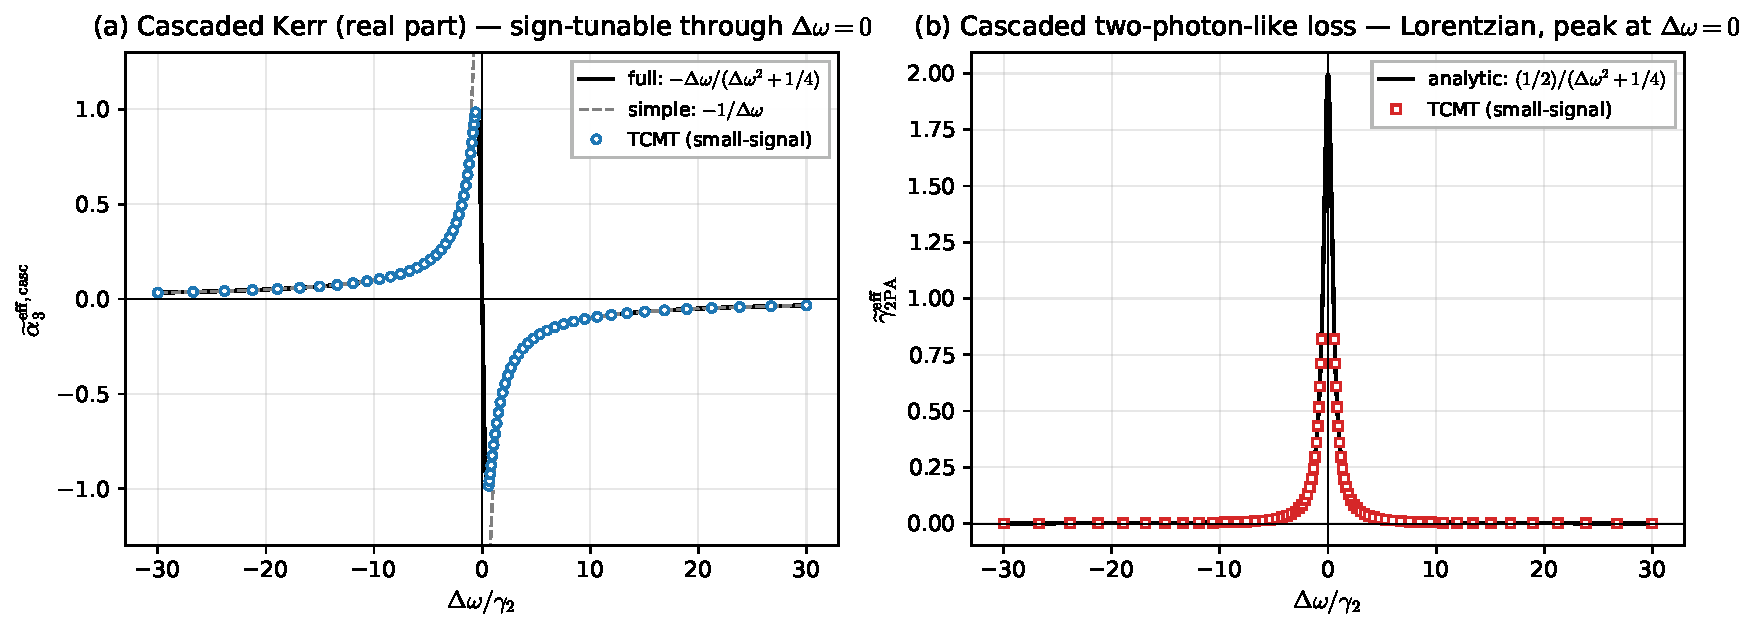
\includegraphics[width=\textwidth]{validation.pdf}
  \caption{Cascaded effective coefficients extracted from steady-state
  TCMT (open markers) compared with closed-form analytic curves (black
  solid). (a)~real (Kerr) part; (b)~imaginary (two-photon-like loss)
  part.}
  \label{fig:validation}
\end{figure}

\paragraph{Parameters.}
$\gamma_1/\gamma_2 = 10$, $\grad/\gamma_1 = 0.5$, $\alpha_3 = 0$,
$\delta_p = 0$; $|s_+| = 10^{-2}$ (small-signal); sweep
$\Dom/\gamma_2 \in [-30,\, 30]$.

\paragraph{Method.}
At each detuning, integrate to steady state and extract the cascaded
contribution from
\begin{equation}
  C \equiv \frac{i\, a_1^{*} a_2}{a_1\, |a_1|^2}
    = -\frac{1}{\gamma_2/2 - i\Dom}
    \;\;\Longrightarrow\;\;
  \alpha^{\effc}_{3,\,{\rm num}} = \mathrm{Im}(C),
  \quad
  \gamma_{2{\rm PA},\,{\rm num}}^{\rm eff} = -\mathrm{Re}(C).
\end{equation}

\paragraph{Panel~(a): cascaded Kerr.}
Numerical TCMT sits exactly on the analytic full form
$\alpha_3^{\effc} = -\Dom/(\Dom^2 + 1/4)$. The simple $-1/\Dom$ form
deviates as $|\Dom| \to \gamma_2/2$ -- the adiabatic-elimination
breakdown of note \S6(i) and \S13(1).

\paragraph{Panel~(b): cascaded TPA.}
A Lorentzian peaked at $\Dom = 0$, FWHM $= \gamma_2$. The loss is the
unavoidable price of resonant enhancement, set entirely by $\gamma_2$
with no analogue in $\mathrm{Im}\,\chithree$.

\paragraph{Takeaway.}
TCMT matches the closed-form expressions to four decimals. The simple
$-1/\Dom$ form, common in cascading literature, underestimates the
true Kerr coefficient by 70\,\% at $\Dom = \gamma_2/2$ and the gap
grows fast as resonance is approached.

% =====================================================================
\subsection{\texorpdfstring{Sign tunability -- walking $\Dom$ through zero}{Sign tunability -- walking Delta-omega through zero}}
\label{sec:sign_flip}

\begin{figure}[H]
  \centering
  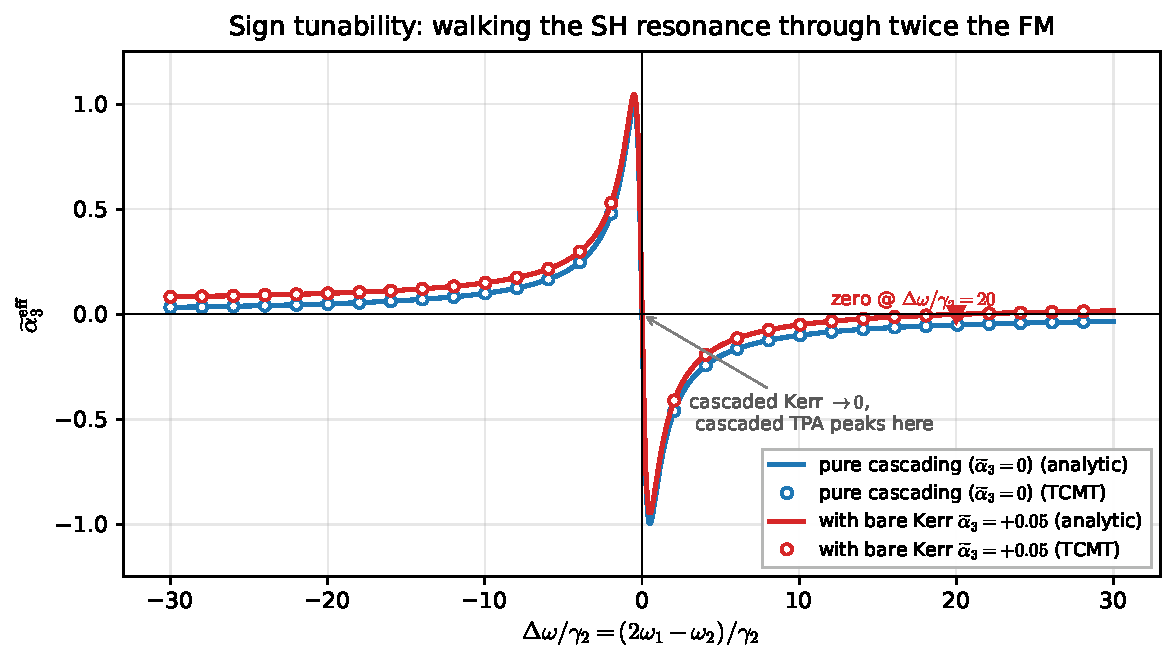
\includegraphics[width=0.85\textwidth]{sign_flip.pdf}
  \caption{Effective Kerr coefficient versus SH detuning. Blue: pure
  cascading. Red: cascading plus a positive bare bulk Kerr; the zero
  of the total response shifts to $\Dom/\gamma_2 = 1/\widetilde\alpha_3 = 20$.
  Grey shading marks the adiabatic-elimination breakdown band.}
  \label{fig:sign_flip}
\end{figure}

\paragraph{Parameters.}
$\gamma_1/\gamma_2 = 10$, $\grad/\gamma_1 = 0.5$, $\delta_p = 0$;
two scenarios for the bare Kerr: $\widetilde\alpha_3 \in \{0,\, +0.05\}$;
sweep $\Dom/\gamma_2 \in [-30,\, 30]$ (excluding $|\Dom| < \gamma_2$).

\paragraph{Why it matters.}
The cascaded Kerr is odd in $\Dom$,
$\alpha_3^{\effc}(-\Dom) = -\alpha_3^{\effc}(\Dom)$. Walking the SH
resonance through $2\omega_1$ -- by tuning the meta-atom geometry,
applying strain, or thermal tuning -- flips the sign of the effective
Kerr from self-defocusing ($\Dom > 0$) to self-focusing ($\Dom < 0$).
With a non-zero bare Kerr, the total zero shifts to
$\Dom = 1/\widetilde\alpha_3$.

\paragraph{Takeaway.}
A single metasurface can deliver self-focusing, self-defocusing, or
cancel native Kerr exactly, by choice of $\Dom$. This was historically
exploited in soliton compression experiments (DeSalvo 1992, Liu 1999).

% =====================================================================
\subsection{Bandwidth--enhancement sum rule}
\label{sec:sumrule}

\begin{figure}[H]
  \centering
  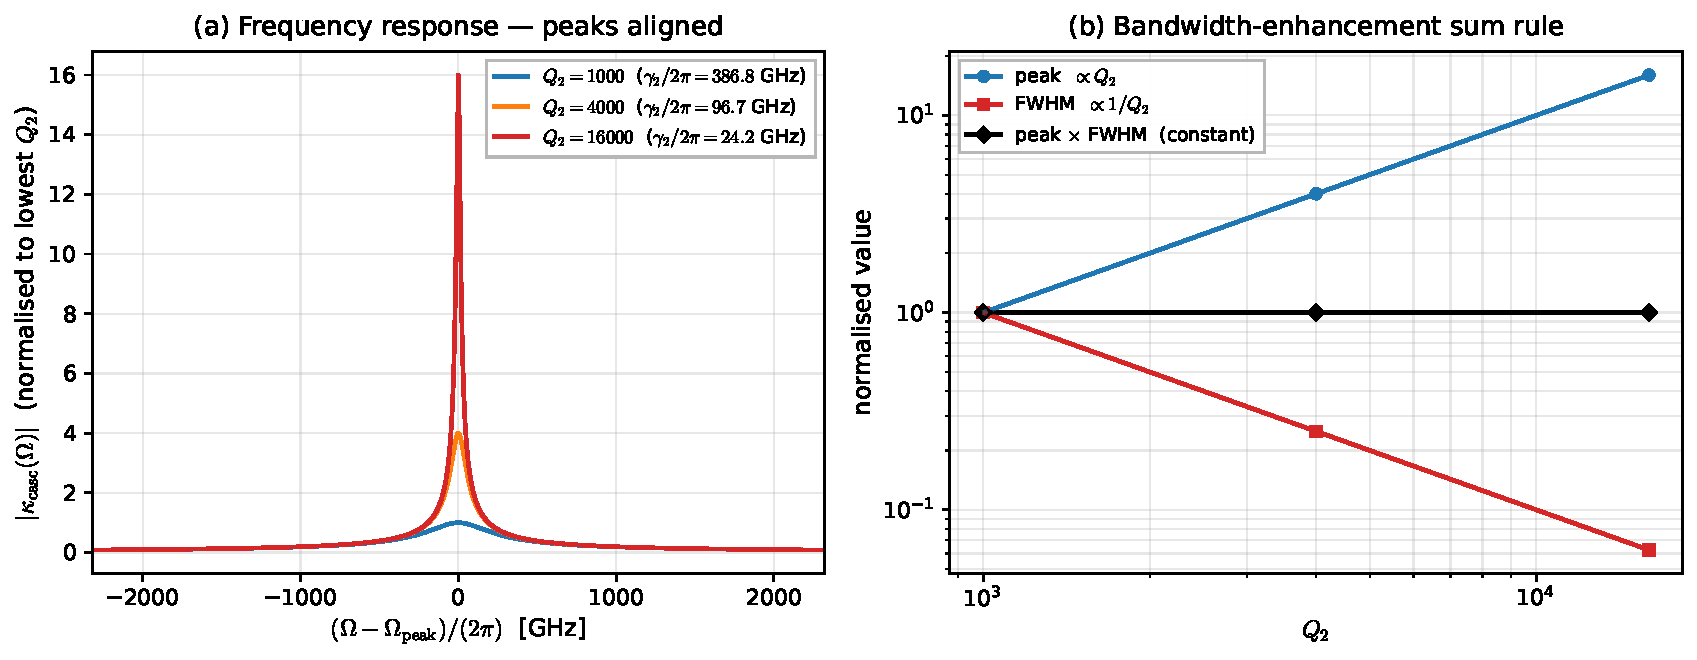
\includegraphics[width=\textwidth]{sum_rule.pdf}
  \caption{(a)~Modulation transfer function $|\kappa_{\rm casc}(\Omega)|$
  evaluated on a shared $\Omega$ grid for three $Q_2$ values, peaks
  aligned at $\Omega = -\DSH$. (b)~Peak grows $\propto Q_2$; FWHM
  shrinks $\propto 1/Q_2$; their product is $Q_2$-independent.}
  \label{fig:sumrule}
\end{figure}

\paragraph{Parameters.}
$\omega_2 = 2\omega_1$, $\omega_1 = 1.22\!\times\!10^{15}$ rad/s
(LiNbO\textsubscript{3}); $Q_2 \in \{1\,000,\, 4\,000,\, 16\,000\}$;
$\Dom = \gamma_2(Q_2{=}4\,000)/2$ chosen so the mid curve sits at the
bandwidth-optimal point; $\Omega$ grid spans $\pm 6\gamma_2^{\max}$
about $\Omega_{\rm peak} = -\Dom$.

\paragraph{Derivation.}
The cascaded modulation transfer function is
$\kappa_{\rm casc}(\Omega) = -|\beta|^2 / [\gamma_2/2 - i(\Omega + \DSH)]$.
At the bandwidth-optimal point $\DSH = \gamma_2/2$,
\begin{equation}
  \text{peak}\, |\kappa| = \frac{|\beta|^2}{\gamma_2/2} \propto Q_2,
  \quad
  \text{FWHM} = \sqrt{3}\, \gamma_2 \propto 1/Q_2,
  \quad
  \text{peak} \times \text{FWHM} = 2\sqrt{3}\, |\beta|^2.
\end{equation}

\paragraph{Numerical verification.}
Peak ratios $[1,\,4,\,16]$, FWHM ratios $[1,\,1/4,\,1/16]$, product
ratios $[1,\,1,\,1]$ to better than $2 \times 10^{-4}$ across the three
$Q_2$ values.

\paragraph{Takeaway.}
Resonant enhancement \emph{redistributes} nonlinear action; it does
not increase the area under the curve. This is the same rule that
limits oscillator-strength sums in linear absorption -- purely
classical, unbreakable by clever resonator design.

% =====================================================================
\section{Cascaded-induced FM dynamics}

\subsection{Bistability: the first experimental fingerprint at the FM}
\label{sec:bistability}

\begin{figure}[H]
  \centering
  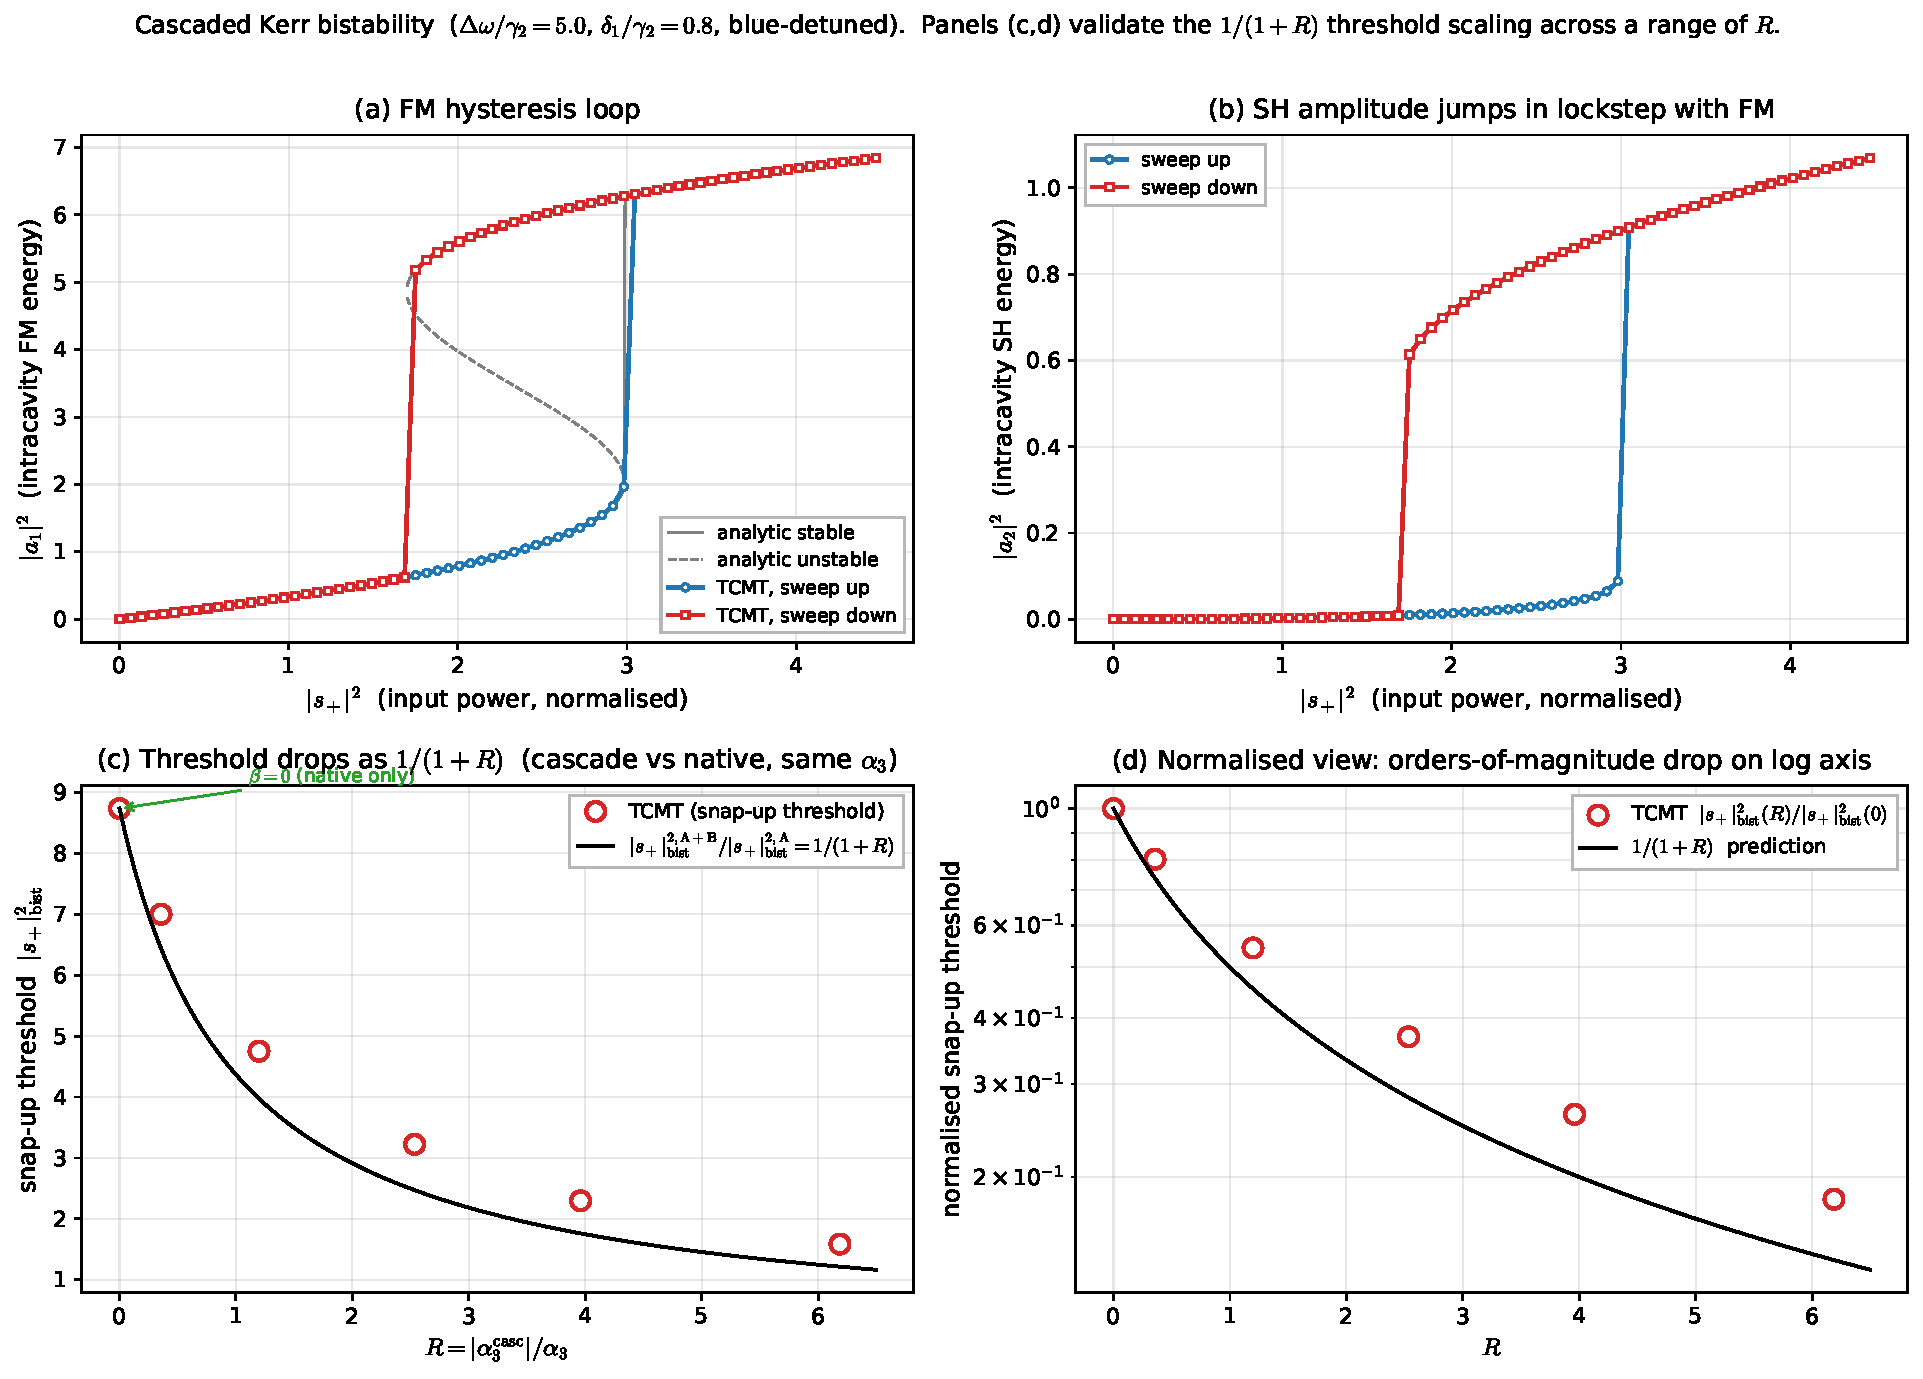
\includegraphics[width=\textwidth]{bistability.pdf}
  \caption{(a)~Hysteresis in the intracavity FM energy under a
  stepwise quasi-static input sweep. The pump is detuned blue of the
  cold-cavity resonance ($\delta_p > 0$) so that the intensity-induced
  red-shift of the dressed FM resonance (negative cascaded Kerr at
  $\Dom > 0$) climbs toward the pump as input grows -- the standard
  geometry for self-defocusing-Kerr bistability. Snap-up at
  $|s_+|^{2} \approx 3.0$, snap-down at $\approx 1.7$; both sit on the
  analytic Kerr+2PA saddle-nodes. (b)~SH amplitude jumps in lockstep
  with the FM, tied by $a_2 = i\beta\, a_1^{2}/(\gamma_2/2 - i\DSH)$.
  (c,d)~Threshold-vs-$R$ sweep at fixed $\Dom$, $\delta_p$, and
  $\alpha_3$ (constructive sign): native Kerr ($\beta=0$) anchors $R=0$;
  increasing $\beta$ adds an aligned cascade contribution
  $\alpha_3^\text{casc}$, raising $R$. TCMT measurements (red) follow
  the predicted $1/(1+R)$ scaling (black) to within $\sim\!30\%$;
  the residual is the cascaded TPA-driven cusp distortion that the
  pure-Kerr $1/(1+R)$ formula does not capture.}
  \label{fig:bistability}
\end{figure}

\paragraph{Parameters.}
$\Dom/\gamma_2 = 5$, $\gamma_1/\gamma_2 = 0.4$, $\grad/\gamma_1 = 0.5$,
$\alpha_3 = 0$, $\delta_p/\gamma_2 = 0.8$ (blue-detuned by
$4 \cdot \gamma_1/2$); 70-step quasi-static sweep with state
continuation, $|s_+|^2 \in [10^{-3},\, 4.5]$, settle time
$t_{\rm s} = 250/\gamma_2$ per step.

\paragraph{Why blue detuning?}
With $\Dom > 0$, $\alpha_3^{\effc} < 0$: the effective FM resonance
shifts down with intensity. To get hysteresis, the pump must sit above
the cold-cavity resonance ($\delta_p > 0$); as input grows, the
shifted resonance climbs toward the pump, the response runs away, and
the system snaps to the upper branch.

\paragraph{Cusp condition.}
From the steady-state cubic
\begin{equation}
  |a_1|^2 \bigl[(g_1 + \gamma_e |a_1|^2)^2 + (\delta_p + \alpha_e |a_1|^2)^2\bigr]
  = \grad\, |s_+|^2,
\end{equation}
with $g_1 = \gamma_1/2$, $\alpha_e = \alpha_3 + \alpha_3^{\effc}$,
$\gamma_e = \gamma_{2{\rm PA}}^{\rm eff}$, the saddle-node fold opens
for $\delta_p > \sqrt{3}\, g_1$. Here $\delta_p = 4 g_1 \gg \sqrt{3} g_1$,
comfortably bistable.

\paragraph{Takeaway.}
A purely monochromatic CW pump can drive the FM through bistability
via cascaded SPM. This is the cleanest signature of cascaded
$\chithree$ at the FM port -- far more sensitive than reflectance
measurements at the SH wavelength.

% =====================================================================
\subsection{Saturation and pump depletion}
\label{sec:saturation}

\begin{figure}[H]
  \centering
  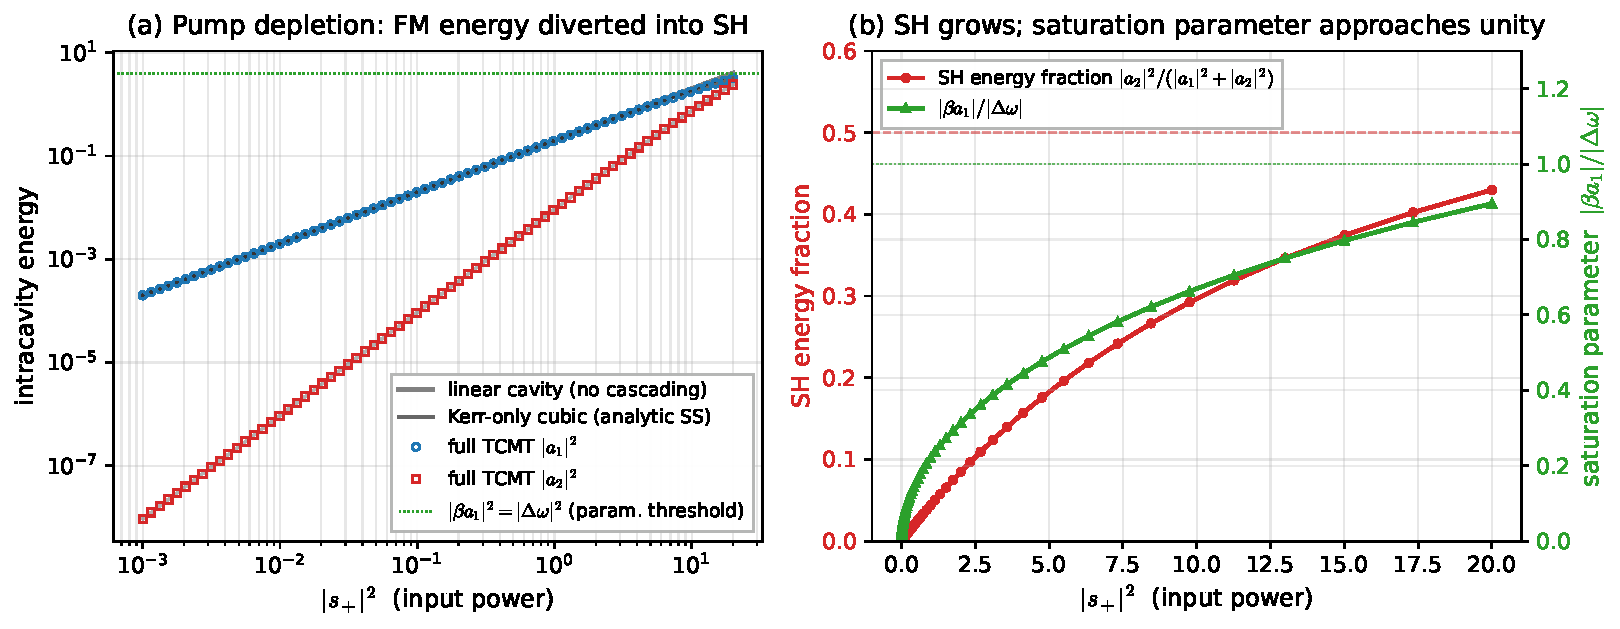
\includegraphics[width=\textwidth]{saturation.pdf}
  \caption{(a)~Log--log of intracavity energies. Linear-cavity
  reference (grey), Kerr-only cubic (black), full TCMT with cascading
  (open markers). The cubic and the TCMT trivial fixed point are
  equivalent to machine precision. (b)~Linear-x view: SH energy
  fraction (red, left) and saturation parameter
  $|\beta a_1|/|\Dom|$ (green, right) climb together.}
  \label{fig:saturation}
\end{figure}

\paragraph{Parameters.}
LiNbO\textsubscript{3} design point of note \S10:
$\Dom/\gamma_2 = 2$, $\gamma_1/\gamma_2 = 10$, $\grad/\gamma_1 = 0.5$,
$\alpha_3 = 0$, $\delta_p = 0$;
70-step state-continuation sweep $|s_+|^2 \in [10^{-3},\, 20]$;
settle time $1500/\gamma_2$ per step.

\paragraph{Why the cap at sat $\approx 1$?}
Past $|\beta a_1| \gtrsim |\Dom|$ the trivial fixed point becomes
parametrically unstable and the deterministic ODE enters a limit
cycle (Section~\ref{sec:parametric_onset}). Below threshold, the
Kerr-only cubic and the full TCMT agree to machine precision -- the
algebraic substitution $a_2 = i\beta\, a_1^{2}/(\gamma_2/2 - i\DSH)$
is exact at any deterministic steady state, with no approximation.

\paragraph{Takeaway.}
The Kerr-equivalent description holds up to
$|\beta a_1| \approx |\Dom|$. Beyond, the FM sees a non-perturbative
back-action -- useful for parametric oscillation, bad for ``the
system as a clean Kerr medium''. The maximum useful $|a_1|^2$ scales
as $1/Q_2$ at fixed $\Dom/\gamma_2$: high-$Q$ devices saturate at
\emph{lower} powers.

% =====================================================================
\subsection{Parametric-oscillation onset above threshold}
\label{sec:parametric_onset}

\begin{figure}[H]
  \centering
  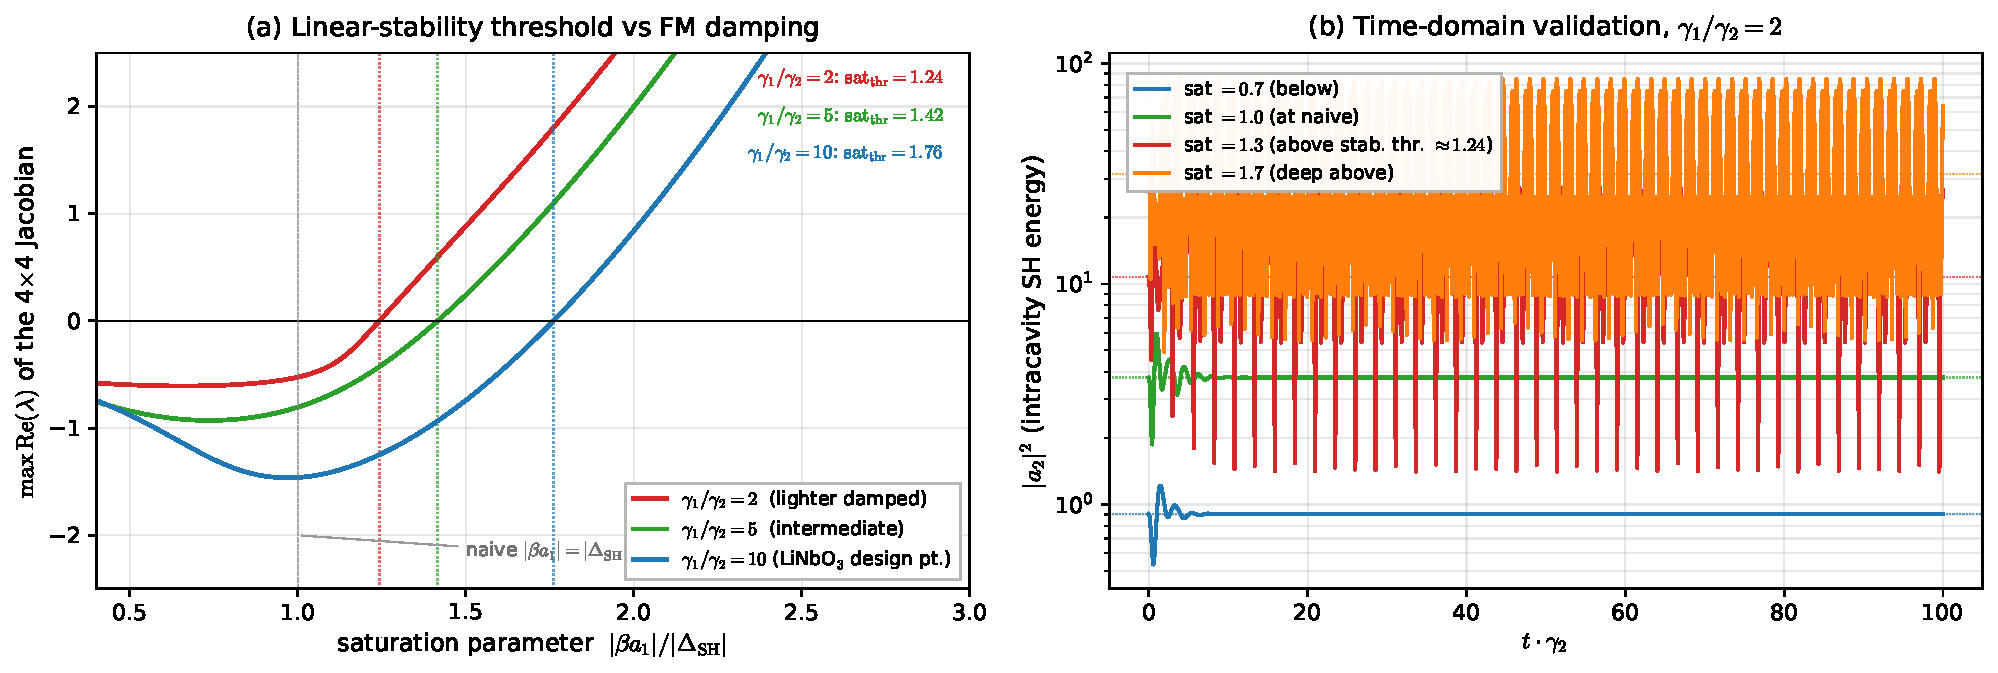
\includegraphics[width=0.95\textwidth]{parametric_onset.pdf}
  \caption{(a)~Largest real part of the 4$\times$4 Jacobian
  eigenvalue of the trivial fixed point versus the saturation
  parameter, for three FM-damping levels. The crossing of zero is the
  parametric-oscillation threshold: $\mathrm{sat}_\mathrm{thr} = 1.24,
  1.42, 1.76$ for $\gamma_1/\gamma_2 = 2,\,5,\,10$ respectively. The
  realistic LiNbO\textsubscript{3} design point
  ($\gamma_1/\gamma_2 = 10$) sits at $\mathrm{sat}_\mathrm{thr}
  \approx 1.76$, well above the naive $|\beta a_1| = |\Dom|$ mark.
  (b)~Time-domain validation at the lighter-damped
  $\gamma_1/\gamma_2 = 2$, chosen so the threshold sits at numerically
  tractable input. Below threshold, a $10^{-3}$ SH perturbation decays
  back to the trivial FP; above threshold, the trajectory enters a
  clear limit cycle. Dotted lines show the trivial-FP values of
  matching colour.}
  \label{fig:parametric_onset}
\end{figure}

\paragraph{Parameters.}
$\Dom/\gamma_2 = 2$, $\gamma_1/\gamma_2 = 2$, $\grad/\gamma_1 = 0.5$,
$\alpha_3 = 0$, $\delta_p = 0$. Lighter FM damping than the realistic
design point so the threshold sits at numerically tractable input.
Four sat parameters $\{0.7,\,1.0,\,1.3,\,1.7\}$, integrated for
$100/\gamma_2$ from $a_2(0) = a_2^{\rm triv} + 10^{-3}\, i$.

\paragraph{Interpretation.}
Above threshold, the trivial fixed point
$a_2 = i\beta a_1^{2}/(\gamma_2/2 - i\DSH)$ has at least one positive
linear-stability eigenvalue. Any perturbation with non-zero projection
on the unstable mode grows exponentially until the nonlinearity clamps
it onto a limit cycle. This is the analogue of the OPO threshold of
note \S13(2). The deterministic ``fixed point'' the saturation figure
plots is metastable.

\paragraph{Takeaway.}
$|\beta a_1| \approx |\Dom|$ is a hard ceiling for the cascaded-Kerr
description -- not because the cubic equation diverges (it does not),
but because the deterministic fixed point loses stability and the
system runs off to a parametric-oscillator regime no Kerr medium can
model.

% =====================================================================
\section{Time-domain consequences}

\subsection{Pulse-bandwidth limit}
\label{sec:pulse_bandwidth}

\begin{figure}[H]
  \centering
  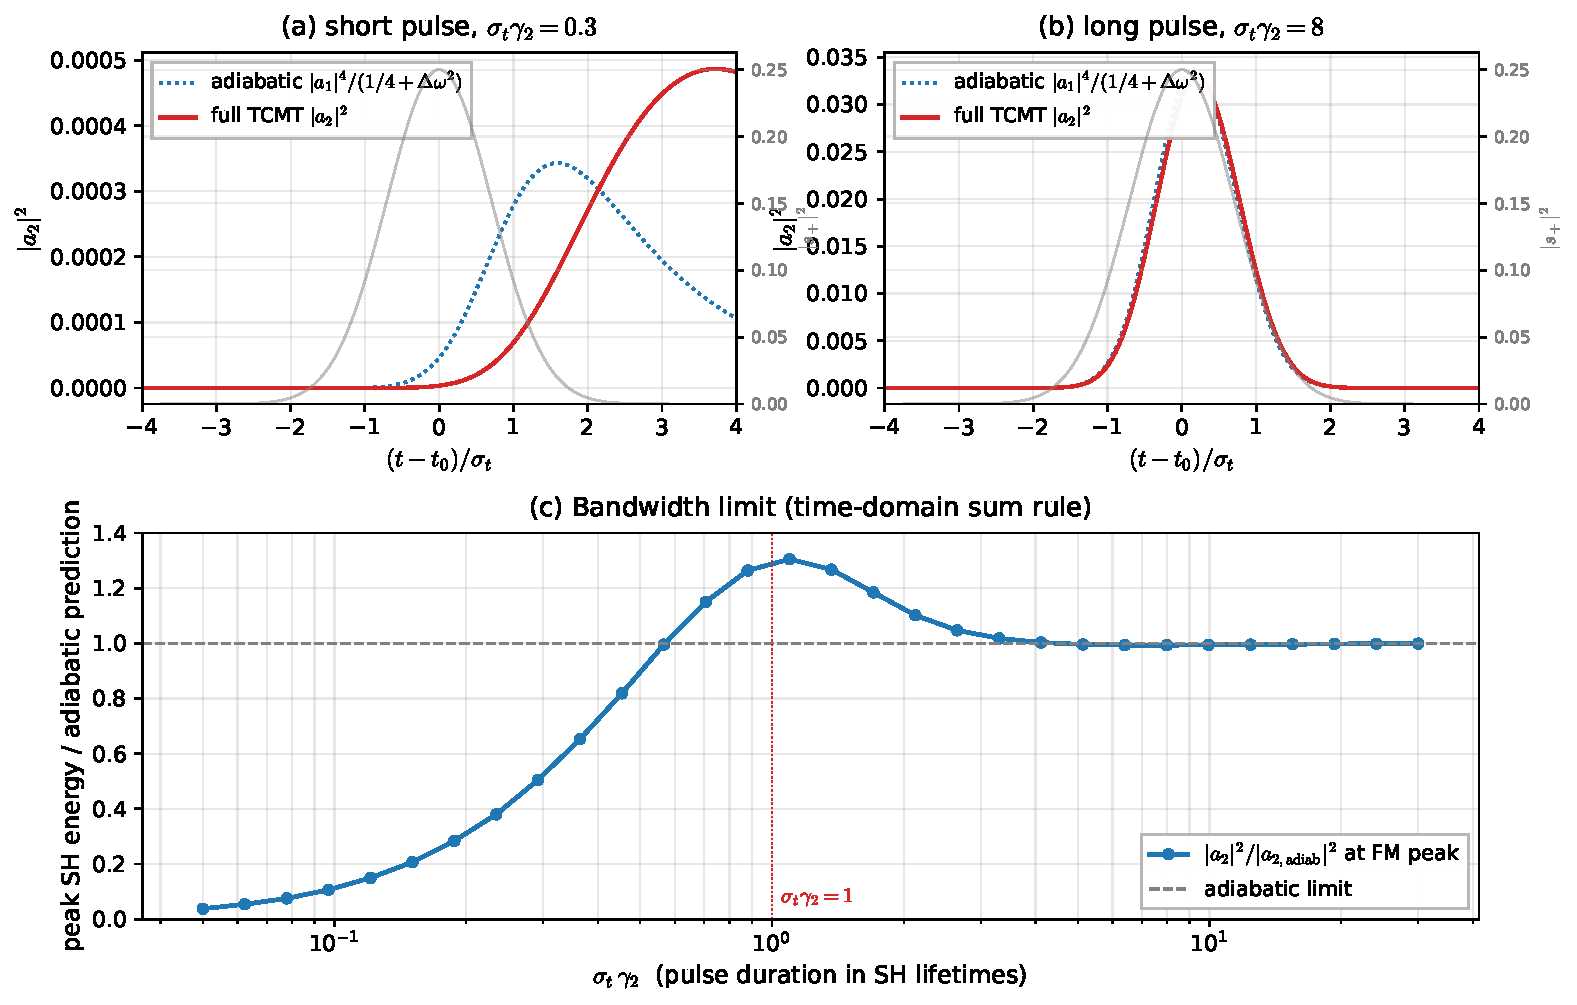
\includegraphics[width=\textwidth]{pulse_bandwidth.pdf}
  \caption{(a)~Short pulse $\sigma_t \gamma_2 = 0.3$: the SH lags and
  undershoots the adiabatic prediction (blue dotted), then rings down
  at rate $\gamma_2/2$. (b)~Long pulse $\sigma_t \gamma_2 = 8$: the SH
  faithfully tracks $|a_1|^{2}$. (c)~Tracking quality at the moment of
  FM peak across $\sigma_t \gamma_2 \in [0.05,\, 30]$. The ratio
  crosses unity at $\sigma_t \gamma_2 \approx 1$ -- the time-domain
  face of the bandwidth--enhancement sum rule -- and overshoots to
  $\sim 1.3$ near $\sigma_t \gamma_2 = 1$ before settling. The
  overshoot is not numerical ringing: at marginal pulse duration the
  FM peaks just before the SH catches up, and the SH receives a brief
  impulsive drive that pushes its peak above the static adiabatic
  value $|a_1|^{4}/(\Dom^{2}+(\gamma_2/2)^{2})$ for an instant.}
  \label{fig:pulse_bandwidth}
\end{figure}

\paragraph{Parameters.}
$\Dom/\gamma_2 = 2$, $\gamma_1/\gamma_2 = 1$, $\grad/\gamma_1 = 0.5$,
$\alpha_3 = 0$, $\delta_p = 0$; Gaussian pump $s_+(t) = s_0\,
\exp[-(t-t_0)^{2}/(2\sigma_t^{2})]$ with $s_0 = 0.5$ for
panels~(a)--(b), $s_0 = 0.3$ for the duration sweep in panel~(c).

\paragraph{Adiabatic prediction.}
Whenever the SH stays slaved to the FM,
$|a_2(t)|^{2} = |a_1(t)|^{4}/[\Dom^{2} + (\gamma_2/2)^{2}]$.

\paragraph{Takeaway.}
Cascaded $\chithree$ enhancement is not ``fast'' Kerr in the
ultrafast sense. For pulse durations shorter than $\sim 1/\gamma_2$
the SH cannot follow and the cascaded contribution rolls off. With
$Q_2 = 4\,000$, $1/\gamma_2 \approx 1.7$ ps; anything sub-picosecond
is too fast.

% =====================================================================
\subsection{Manley--Rowe / energy-conservation check}
\label{sec:manley_rowe}

\begin{figure}[H]
  \centering
  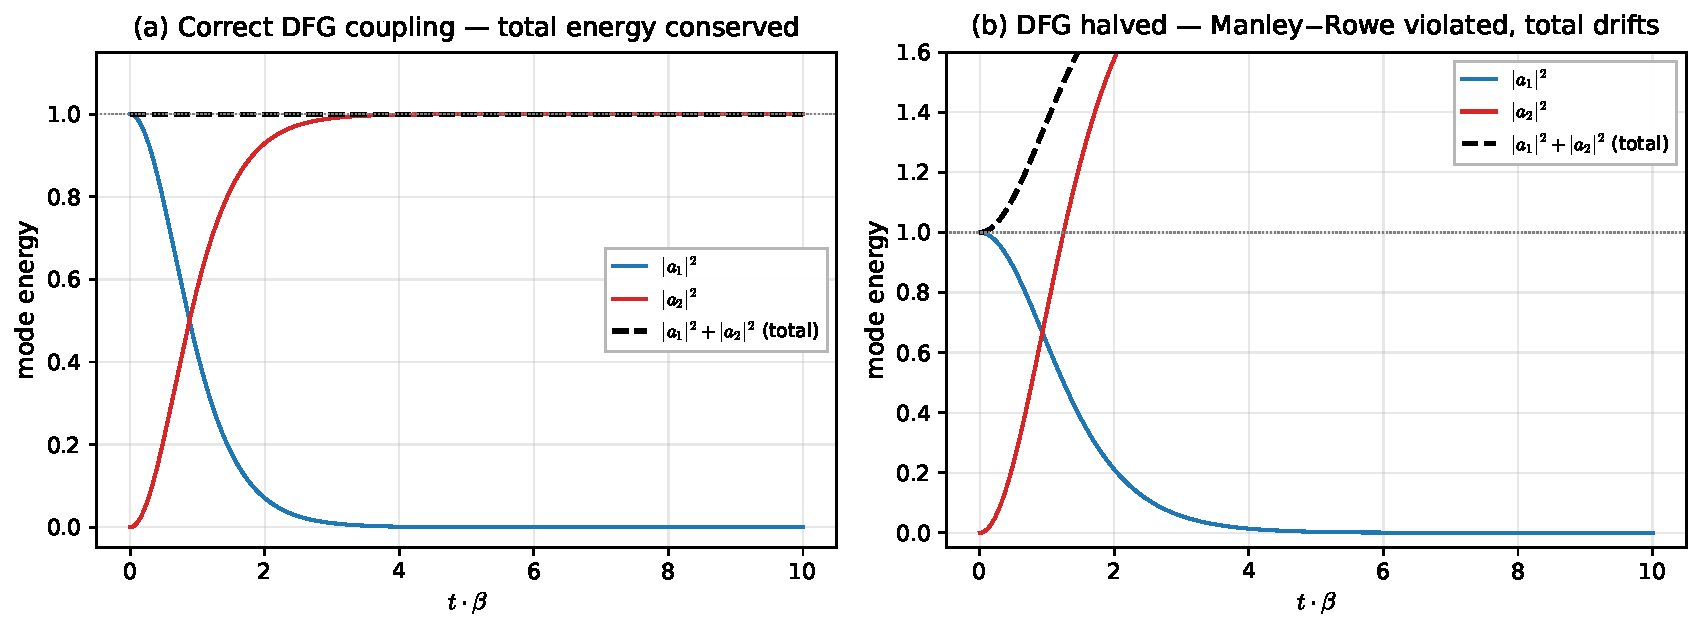
\includegraphics[width=\textwidth]{manley_rowe.pdf}
  \caption{Lossless TCMT, no input. (a)~Correct DFG factor: total
  energy stays at 1.0 to machine precision. (b)~Halved DFG (the
  ``$\kappa$ vs $\kappa/2$'' bug of the original derivation): total
  energy grows past 1.6 by $t = 2/\beta$ -- energy created out of
  nothing.}
  \label{fig:manley_rowe}
\end{figure}

\paragraph{Parameters.}
$\gamma_1 = \gamma_2 = 0$ (lossless), $s_+ = 0$ (no input),
$\Dom = 0$ (degenerate, fastest exchange);
initial state $(a_1, a_2) = (1, 0)$; integration window
$t \cdot \beta \in [0,\, 10]$.

\paragraph{Why this matters.}
Manley--Rowe in the lossless limit demands
$\frac{d}{dt}(|a_1|^{2} + |a_2|^{2}) = 0$, equivalently
$\beta^{(1)} = \beta^{*}$: a single coupling constant on both sides,
not two independent ones. This is built in by the factor of 2 in the
DFG polarisation
$P^{(2)}(\omega_1) = 2\eps_0\, \chitwo\, E(2\omega_1)\, E^{*}(\omega_1)$
that note \S2 rederives.

\paragraph{Numerical drifts.}
Correct: total-energy drift over $10/\beta$ time units is
$1.4 \times 10^{-14}$ (machine precision).
Halved DFG: drift $= 1.0$, the same order of magnitude as the total
energy itself.

\paragraph{Takeaway.}
The factor-of-2 the note rederives is not a cosmetic fix -- without
it, the model violates the second law. Any TCMT code that drops it is
silently wrong; this figure is the smoke test.

% =====================================================================
\section{Design space}

\subsection{Bulk PPLN versus metasurface: the same sum rule, different operating point}
\label{sec:bulk}

\begin{figure}[H]
  \centering
  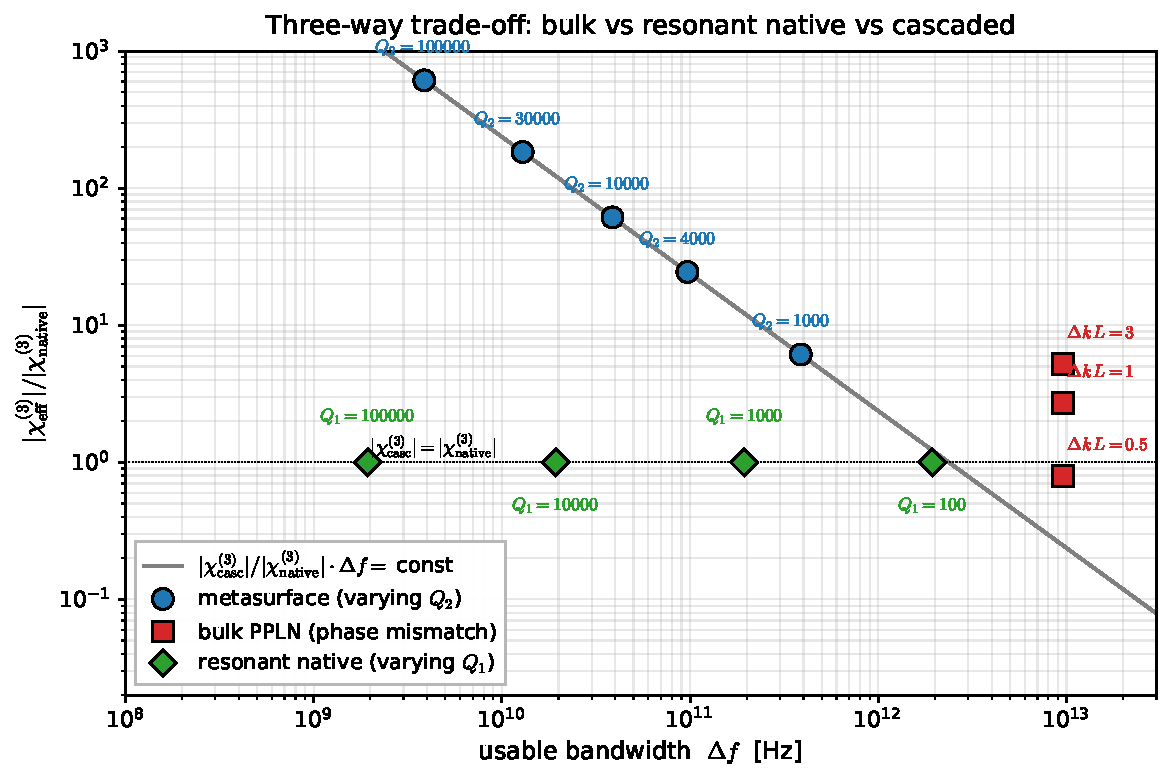
\includegraphics[width=0.92\textwidth]{bulk_vs_metasurface.pdf}
  \caption{Enhancement
  $|\chithree_{\rm casc}|/|\chithree_{\rm native}|$ versus usable
  bandwidth in lab units. Circles: doubly-resonant metasurface,
  varying $Q_2$. Squares: bulk phase-mismatched PPLN. Both regimes lie
  on the common sum-rule hyperbola defined by the same
  $|\chitwo|^{2}\eta_\geom/n_2^{2}$.}
  \label{fig:bulk}
\end{figure}

\paragraph{Parameters.}
LiNbO\textsubscript{3}: $\omega_1 = 1.22\!\times\!10^{15}$ rad/s,
$|\chitwo| = 5\!\times\!10^{-11}$ m/V, $|\chithree|_{\rm native} =
2\!\times\!10^{-21}$ m$^{2}$/V$^{2}$, $n_2 = 2.26$,
$\eta_\geom = 0.3$.
Metasurface points: $Q_2 \in \{10^{3},\,4\!\times\!10^{3},\,10^{4},\,
3\!\times\!10^{4},\,10^{5}\}$.
Bulk PPLN points: $\Delta k\, L \in \{0.5,\,1,\,3\}$, $\Delta f \approx 1$ THz.

\paragraph{Formulas.}
The metasurface enhancement, evaluated at fixed
$\Dom/\gamma_2$ via eq.~(\ref{eq:chi3casc}):
\begin{equation}
  \text{enh}(\Dom/\gamma_2)
   = \frac{Q_2}{n_2^{2}}\,
     \frac{(\Dom/\gamma_2)^{-1}}{6}\,
     \frac{\eta_\geom\, |\chitwo|^{2}}{|\chithree|_{\rm native}},
   \quad
   \Delta f = \frac{\gamma_2}{2\pi} = \frac{2\omega_1}{2\pi Q_2}.
\end{equation}
Two natural operating points (Table~\ref{tab:opppoint}): the
bandwidth-optimal $\Dom = \gamma_2/2$ (peak of
$|\alpha_3^{\effc}|$ in Fig.~\ref{fig:validation}a) and the
``conservative'' $\Dom = 2\gamma_2$, where saturation is pushed up by
$4\times$ at the cost of $4\times$ lower enhancement.
The bulk regime uses the SVEA Stegeman/DeSalvo result
\begin{equation}
  \chithree_{\text{casc,bulk}}
   = -\frac{2\,\omega_1}{3\,c\,n_2\,\Delta k}\,
       |\chitwo|^{2}\, F(\Delta k\,L),
   \quad
   F(x) \equiv 1 - \frac{\sin x}{x}\,e^{-ix},
\end{equation}
with bandwidth $\Delta f \sim |\Delta k|\, v_g / (2\pi) \sim$ few THz.
(Note: only the SH-mode index $n_2$ appears; the powers of $n_1$ from the
FM SVEA projection cancel against $n_1$ in the cascade kernel, paralleling
the metasurface single-resonance result.  See main note eq.~(chi3casc-bulk).)

\begin{table}[H]
\centering
\renewcommand{\arraystretch}{1.20}
\small
\begin{tabular}{lcccc}
\toprule
$\Dom/\gamma_2$ & prefactor & $R(Q_2{=}4\,000)$ & $R(Q_2{=}10^{4})$ & $\Delta f$ [GHz] \\
\midrule
$1/2$ (BW-optimal)      & $Q_2/(6\, n_2^{2})$  & $49$ & $122$ & $97$ \\
$1$ (edge of adiabatic) & $Q_2/(12\, n_2^{2})$ & $25$ & $61$  & $97$ \\
$2$ (conservative)      & $Q_2/(24\, n_2^{2})$ & $12$ & $30$  & $97$ \\
\bottomrule
\end{tabular}
\caption{Cascaded-$\chithree$ enhancement at three operating points,
LiNbO\textsubscript{3} at telecom ($n_2 = 2.26$, $\eta_\geom = 0.3$,
$|\chitwo| = 5\!\times\!10^{-11}$ m/V,
$|\chithree|_\text{native} = 2\!\times\!10^{-21}$ m$^{2}$/V$^{2}$,
$\gamma_2 = \omega_2/Q_2 = 2\omega_1/Q_2$).  $\Delta f = \gamma_2/(2\pi)$
quoted at $Q_2 = 4\,000$; it depends on $Q_2$, not on $\Dom$. The
summary table and Fig.~\ref{fig:bulk} use the conservative point
throughout for consistency; the $\Dom=\gamma_2$ row is included
because the often-quoted ``$R\!\sim\!25$ for LiNbO$_3$'' figure
originates there, at the edge of adiabatic validity.}
\label{tab:opppoint}
\end{table}

Sum-rule constant from the metasurface family at the conservative
operating point:
$\text{enh} \cdot \Delta f({\rm Hz}) = 1.16\!\times\!10^{12}$.
Pulling $\Dom$ down to $\gamma_2$ doubles the constant
(at the cost of edge-of-adiabatic operation); pulling further to
$\gamma_2/2$ doubles again.  The hyperbola is the same; only its
absolute height shifts.

\paragraph{Trade-off.}
With the corrected $1/n_2$ scaling, the bulk PPLN $|\chithree_{\rm casc}|$
in LiNbO$_3$ at $\Delta k\!=\!3\!\times\!10^{5}$~m$^{-1}$ is
$\sim\!10^{-20}$~m$^2$/V$^2$, roughly $5\times$ native -- not
``comparable'' to native as the earlier draft claimed.  The
metasurface at $Q_2=4{,}000$ delivers $\sim 25\times$ native at the
bandwidth-optimal point ($\Delta\omega=\gamma_2/2$) or $\sim 12\times$
at the conservative operating point ($\Delta\omega=2\gamma_2$),
so the metasurface still wins the $|\chithree|$ comparison by
$\sim 2\text{--}5\times$ at routine $Q_2$.  In the
$|\chithree|\cdot\Delta f$ product, however, bulk leads by $\sim 20$--$40\times$
because its $\sim 10$~THz bandwidth dwarfs the cascade's $\lesssim 100$~GHz
bandwidth.  The metasurface trades $\sim 0.5\text{--}1$ order of magnitude
in $|\chithree_{\rm eff}|$ for $\sim 2\text{--}3$ orders of magnitude in
bandwidth.  Both regimes are best-in-class for their respective
applications: high-$Q$ metasurfaces for CW-pumped bistability,
parametric thresholds, and frequency-comb stabilisation;
bulk phase-mismatched PPLN for ultrafast soliton compression and
broadband all-optical switching.

% =====================================================================
\subsection{Geometric overlap is the binding constraint}
\label{sec:overlap}

\begin{figure}[H]
  \centering
  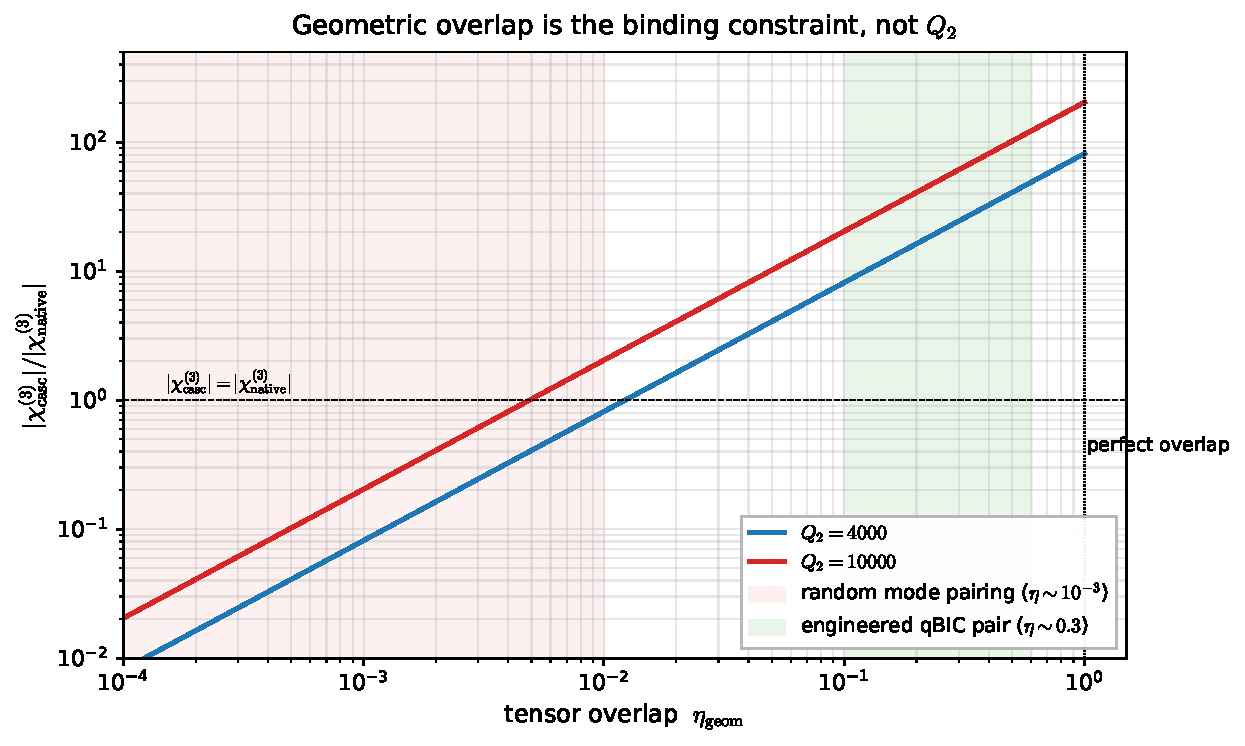
\includegraphics[width=0.92\textwidth]{overlap_eta.pdf}
  \caption{Cascaded enhancement versus tensor overlap $\eta_\geom$ on
  log--log, for two $Q_2$ values. Random mode pairing
  ($\eta_\geom \sim 10^{-3}$, red shaded) gives sub-native cascading
  even at $Q_2 = 10^{4}$. Engineered qBIC pair
  ($\eta_\geom \sim 0.3$, green shaded) recovers $25$--$60\times$
  enhancement.}
  \label{fig:overlap}
\end{figure}

\paragraph{Parameters.}
LiNbO\textsubscript{3} numbers as above; $Q_2 \in \{4\,000,\,10\,000\}$;
$\eta_\geom \in [10^{-4},\,1]$ on a log grid; vertical bands at
$\eta_\geom \sim 10^{-3}$ (random pairing) and $\eta_\geom \sim 0.3$
(engineered qBIC).

\paragraph{Conditions for non-vanishing overlap (note \S8).}
The integral
$\eta_\geom \propto \big|\int \chitwo_{ijk}(\ri)\, f_{2,i}^{*}\, f_{1,j}\, f_{1,k}\,\dthreer\big|^{2}$
vanishes unless three conditions hold simultaneously:
\begin{enumerate}[nosep]
  \item No bulk inversion symmetry in the meta-atom material
        (LiNbO\textsubscript{3}, GaAs, GaP, AlGaAs all qualify).
  \item Mode-symmetry mismatch is lifted: if both modes share parity
        under all spatial symmetries, the integrand has definite
        parity that may force the integral to zero. Quasi-BIC
        engineering breaks one such symmetry while preserving high
        $Q_2$.
  \item Adequate radial overlap of $f_2$ with $f_1^{2}$ at the
        unit-cell scale.
\end{enumerate}

\paragraph{Takeaway.}
$Q_2$ alone buys nothing if $\eta_\geom$ is small. A factor-of-$2.5$
in $Q_2$ shifts the line by $\sim 0.4$ dex; a factor-of-$100$
reduction in $\eta_\geom$ shifts it 2 dex \emph{down}. Geometry
first; resonance $Q$ second.

% =====================================================================
\subsection{\texorpdfstring{Refractive-index dependence: $1/n_2^{2}$, not $1/n^{3}$}{Refractive-index dependence: 1/n2 squared, not 1/n cubed}}
\label{sec:n2}

\begin{figure}[H]
  \centering
  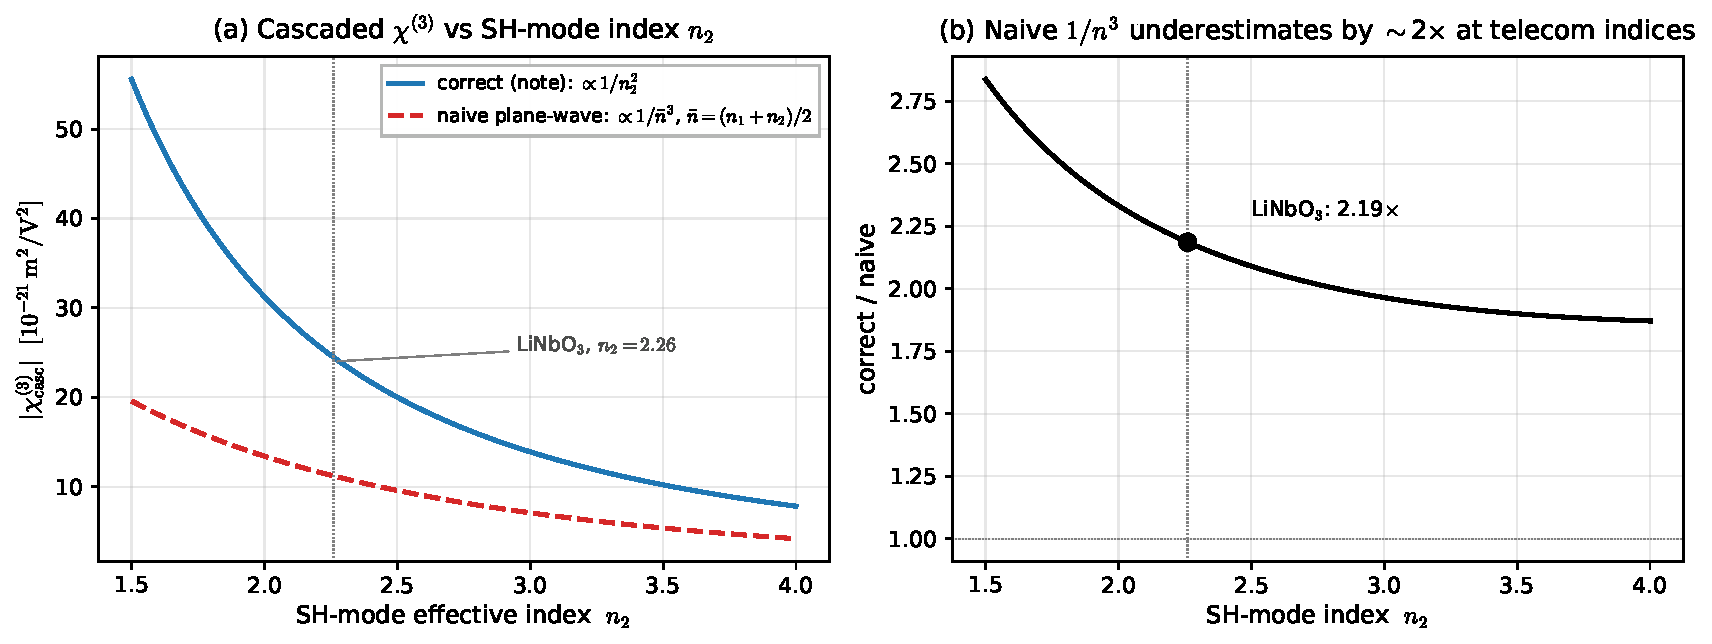
\includegraphics[width=\textwidth]{n2_scaling.pdf}
  \caption{(a)~$|\chithree_{\rm casc}|$ versus SH-mode index $n_2$ at
  fixed $Q_2 = 4\,000$, $\eta_\geom = 0.3$. The resonant single-mode
  result~(\ref{eq:chi3casc}) (blue) versus the bulk plane-wave
  $1/\bar n^{3}$ form (red, with $\bar n = (n_1+n_2)/2$).
  (b)~Their ratio. At LiNbO\textsubscript{3} ($n_2 = 2.26$) the ratio
  is $2.19$, matching $\bar n^{3}/n_2^{2} = 2.18$. The figure is
  comparing two derivations side-by-side, not validating one against
  the other: the bulk form is incorrect for resonant single-mode
  cascading because the four powers of $n_1$ do not appear in the
  bulk derivation.}
  \label{fig:n2}
\end{figure}

\paragraph{Parameters.}
$Q_2 = 4\,000$, $\Dom = 2\gamma_2$, $\eta_\geom = 0.3$,
$|\chitwo| = 5 \!\times\! 10^{-11}$ m/V; sweep $n_2 \in [1.5,\,4]$
with $n_1 = 2.21$ fixed; the naive ``single-index'' form uses
$\bar n = (n_1 + n_2)/2$.

\paragraph{Why $n_1$ cancels.}
The $f_2{:}f_1 f_1$ overlap integral has dimension
$|\chitwo|/(\eps_0^{3/2}\, n_2\, n_1^{2}\, \sqrt{V_{\rm eff}})$.
The $\int |\f_1|^{4}\dthreer$ in the denominator scales as
$1/(\eps_0^{2}\, n_1^{4}\, V_{\rm eff})$. Their ratio leaves only
$n_2^{2}$. Modes in higher-index material concentrate \emph{less}
field per unit stored energy, so the $f_2{:}f_1 f_1$ coupling is
suppressed by $1/n_2$, but the FM-mode normalisation symmetrically
draws power from both ends.

\paragraph{Takeaway.}
A non-trivial correction over the original derivation; particularly
important when comparing with experiment, where measured
$\chithree_{\rm casc}$ rarely matches the ``obvious'' $1/n^{3}$
scaling.

% =====================================================================
\subsection{Power-resolved transmission lineshape}
\label{sec:transmission}

\begin{figure}[H]
  \centering
  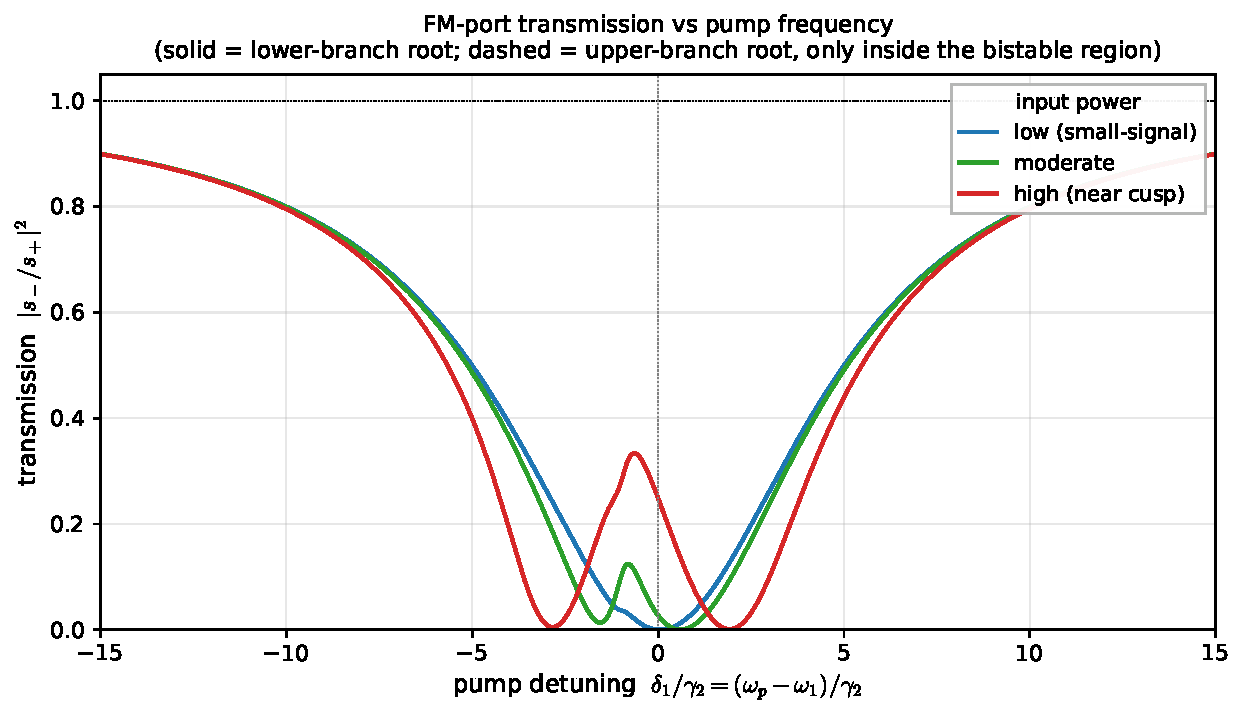
\includegraphics[width=\textwidth]{transmission_lineshape.pdf}
  \caption{FM-port transmission $|s_-/s_+|^{2}$ versus pump detuning
  $\delta_p/\gamma_2$ at three input powers. The low-power curve is
  a clean critically-coupled Lorentzian dip; the high-power curve
  shows the lineshape distortion through cascaded Kerr self-detuning
  combined with the sign flip of $\alpha_3^{\effc}$ as $\DSH$ crosses
  zero, producing the characteristic double-dip pattern unique to a
  doubly-resonant cascaded system.}
  \label{fig:transmission}
\end{figure}

\paragraph{Parameters.}
$\Dom/\gamma_2 = 2$, $\gamma_1/\gamma_2 = 10$, $\grad/\gamma_1 = 0.5$,
$\alpha_3 = 0$. Three input levels, $|s_+|^{2} \in \{0.5,\,10,\,60\}$
(``low / moderate / near cusp''). Pump detuning swept across
$\delta_p/\gamma_2 \in [-15,\, 15]$. At each $\delta_p$, the cubic
roots are evaluated and the transmission constructed from
$a_1 = \sqrt{\grad}\, s_+ / [g_1 + \gamma_e |a_1|^{2}
   - i(\delta_p + \alpha_e |a_1|^{2})]$.

\paragraph{Two competing effects.}
\begin{enumerate}[nosep]
  \item \emph{Self-detuning from cascaded Kerr.} With
        $\alpha_3^{\effc} < 0$ at $\DSH > 0$, the effective FM
        resonance walks blue with intensity. The dip pulls toward
        $+\delta_p$.
  \item \emph{Sign flip across $\DSH = 0$.} Sweeping $\delta_p$ also
        sweeps $\DSH = 2\delta_p + \Dom$. At $\delta_p = -\Dom/2 = -1$
        the cascaded coefficient changes sign and the response goes
        from self-defocusing to self-focusing. The high-power red
        curve has two dips (one on each side of $\DSH = 0$) and a
        transmission peak in between.
\end{enumerate}

\paragraph{Takeaway.}
For practical metrology of cascaded $\chithree$, a power-swept
transmission scan is the most diagnostic single experiment. Low-power
Lorentzian gives $\gamma_1$ and $\grad/\gamma_1$; the high-power
lineshape encodes $\beta$, $\Dom$, and the sign-flip-induced double
dip. The bistability cusp is read off the same scan.

% =====================================================================
\section{Cascaded vs.\ native: architectural comparison}\label{sec:comparison}

This section numerically validates Section~11 of the main note, which
poses the question: is the cascaded $\chitwo{:}\chitwo$ route actually
preferable to engineering a single high-$Q$ resonance that enhances the
material's \emph{native} bulk $\chithree$? Both architectures use a
high-$Q$ FM cavity at $\omega_1$ to build up intracavity intensity;
they differ in what the cavity then turns that intensity into.

Within the TCMT framework, the two architectures are limits of the
\emph{same} model: native sets $\beta = 0$ (the SH decouples), cascaded
keeps $\beta = 1$ and the SH is co-resonant near $2\omega_1$. The bare
Kerr $\alpha_3$ can be present in both. The five figures below stress
the comparison along complementary axes: TCMT response curves; the
material-dependent enhancement ratio $R$; the 1-D phase-bandwidth
locus; the 2-D design landscape; and the loss penalty cascaded carries
that native does not.

% --------------------------------------------------------------
\subsection{Side-by-side TCMT response}\label{sec:archresponse}

\begin{figure}[H]
  \centering
  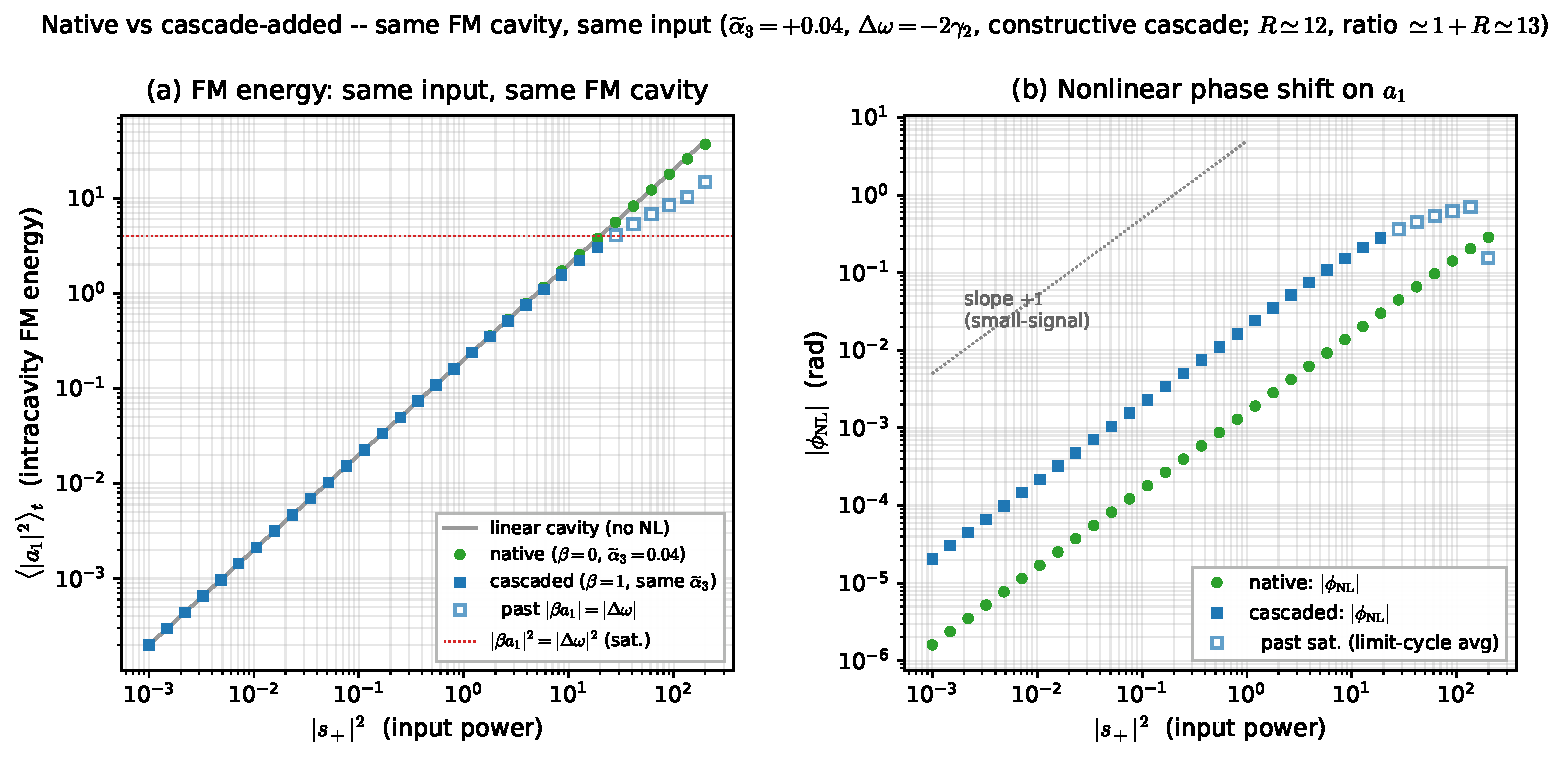
\includegraphics[width=\textwidth]{arch_response.pdf}
  \caption{Direct TCMT comparison of the two architectures under
  identical CW input and identical FM cavity. (a) Intracavity FM
  energy $|a_1|^{2}$ vs.\ input power: native sits on the linear-cavity
  reference (its tiny bare Kerr barely deflects it); cascade peels
  below and saturates at $|a_1|^2 \to |\Dom|^2$. (b) Magnitudes of the
  nonlinear phase shift on $a_1$. At small signal, the cascade phase
  is $\sim 12\times$ larger than the native phase, matching the
  predicted ratio $R = 12$ (LiNbO\textsubscript{3} conservative
  operating point, $\Dom = 2\gamma_2$, factor-24 prefactor) within a
  few percent.}
  \label{fig:archresponse}
\end{figure}

\paragraph{What is plotted.}
Both architectures share the same FM cavity ($\gamma_1, \grad$) and
identical input $s_+$ on resonance ($\delta_p = 0$). The native run
uses $\beta = 0$ (no SH coupling); cascaded uses $\beta = 1$ and
$\Dom = 2\gamma_2$. Both runs carry the same bare Kerr
$\widetilde\alpha_3 = 0.04$, the LiNbO\textsubscript{3} dimensionless
native Kerr at the worked-example operating point ($\Dom = 2\gamma_2$,
$Q_2 = 4{,}000$; calibrated so $|\alpha_3^{\rm eff,casc}|/\alpha_3 =
R \approx 12$, see \S\ref{sec:setup}).  For each $|s_+|^{2} \in
[10^{-3}, 200]$ we integrate to steady state with state continuation
and extract $|a_1|^{2}$, $|a_2|^{2}$, and the phase
$\phi_{\rm NL}=\arg(a_1)$.

\paragraph{Parameters.}
$\Dom/\gamma_2 = 2$, $\gamma_1/\gamma_2 = 10$, $\grad/\gamma_1 = 0.5$,
$\widetilde\alpha_3 = 0.04$ (LiNbO\textsubscript{3} dimensionless
native Kerr at the conservative operating point $\Dom = 2\gamma_2$,
$Q_2 = 4{,}000$; chosen so $\alpha_3^{\rm eff,casc}/\alpha_3
\approx 12$ matches the worked-example $R$ of
Section~\ref{sec:hostsurvey}), $\delta_p = 0$.

\paragraph{Result.}
Numerically, $|\phi_{\rm cas}/\phi_{\rm nat}|_{|s_+|^2 = 1} \approx
12$, matching the analytic $R \approx 12$ from the explicit form
\eqref{eq:chi3casc} at $\Dom = 2\gamma_2$ within a few percent.  The
residual deficit is the small ($\sim 6\%$) $\gamma_2/2$ correction to
the simple $-1/\Dom$ form: at $\Dom = 2\gamma_2$, the full Kerr
coefficient is $\Dom/(\Dom^2 + (\gamma_2/2)^2) = 0.471$ vs.\ the
simple $1/\Dom = 0.5$, exactly $-5.8\,\%$.  The cascaded curve clearly
saturates near $|s_+|^{2} \sim 30$ where the FM enters the
parametric-instability regime studied in
Section~\ref{sec:parametric_onset}.

\paragraph{Interpretation.}
At small signal the ratio of the cascaded to native phase shifts is
exactly the structural enhancement $R$, independent of $Q_1$. Pushing
$Q_1$ higher boosts \emph{both} curves equally (the FM cavity is the
common factor), so the comparison really is between the two material
coefficients $\alpha_3^{\effc}$ and $\alpha_3^{\rm nat}$. At high
power the cascaded curve flattens because of saturation -- the
fundamental limitation of cascading that native does not share.

% --------------------------------------------------------------
\subsection{\texorpdfstring{Cross-host material survey: the enhancement ratio $R$}{Cross-host material survey: the enhancement ratio R}}\label{sec:hostsurvey}

\begin{figure}[H]
  \centering
  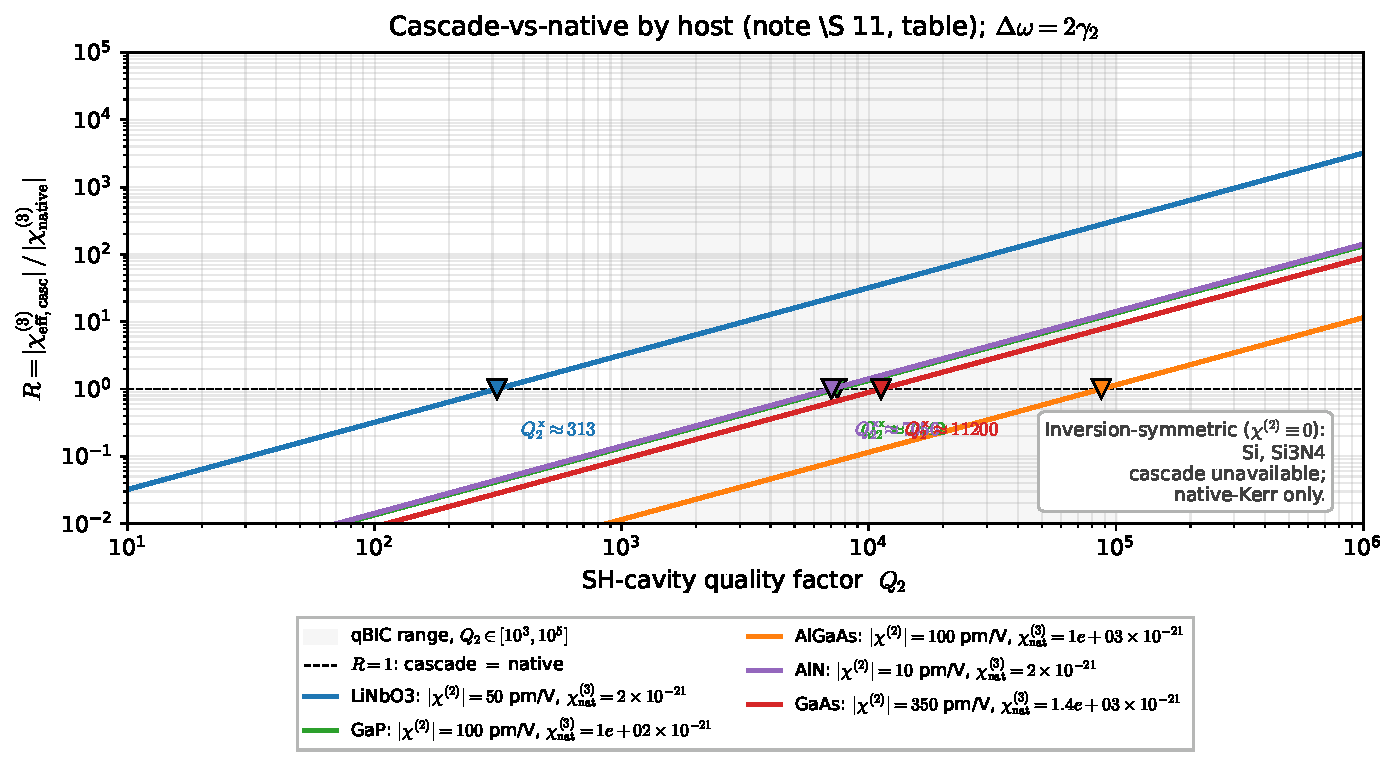
\includegraphics[width=0.92\textwidth]{cascaded_vs_native.pdf}
  \caption{Cascaded enhancement ratio $R(Q_2)$ for five non-centrosymmetric
  hosts, log--log. Native sits on the dashed line at $R = 1$.
  Crossover markers ($\nabla$) indicate $Q_2^{\rm crossover}$ at which
  $R = 1$ for each host. Inversion-symmetric hosts (Si, Si$_3$N$_4$)
  have no cascade route: $\chitwo \equiv 0$.}
  \label{fig:hostsurvey}
\end{figure}

\paragraph{What is plotted.}
The dimensionless enhancement ratio
\begin{equation}
  R(Q_2) \equiv
  \frac{|\chithree_{\rm eff,casc}|}{|\chithree_{\rm native}|}
  = \frac{Q_2}{24\, n_2^{2}}\,
    \frac{\eta_\geom\, |\chitwo|^{2}}{|\chithree_{\rm native}|},
  \label{eq:Rdef}
\end{equation}
linear in $Q_2$ at fixed $\Dom/\gamma_2 = 2$ and $\eta_\geom = 0.3$.
The factor $1/24$ comes from $\omega_1/\Dom = Q_2/4$ at the
conservative operating point $\Dom = 2\gamma_2 = 4\omega_1/Q_2$.
Crossover Q given by $R = 1$:
\begin{equation}
  Q_2^{\rm crossover} = \frac{24\, n_2^{2}\, |\chithree_{\rm native}|}
                              {\eta_\geom\, |\chitwo|^{2}}.
\end{equation}
Hosts: LiNbO\textsubscript{3}, GaP, AlGaAs, AlN, GaAs (cascade
available); Si, Si\textsubscript{3}N\textsubscript{4}
(centrosymmetric, $\chitwo \equiv 0$, cascade unavailable).

\paragraph{Parameters.}
Telecom $\lambda_1 = 1.55$\,\textmu m, $\eta_\geom = 0.3$, $Q_2$ swept
log-uniform across $[10,\,10^{6}]$. Per-host $\chitwo$, $\chithree$,
$n$: see Table~\ref{tab:hosts}.

\begin{table}[H]
\centering
\small\renewcommand{\arraystretch}{1.15}
\begin{tabular}{lcccc}
\toprule
Host & $|\chitwo|$ [m/V] & $|\chithree_{\rm native}|$ [m$^{2}$/V$^{2}$]
     & $n$ & $Q_2^{\rm crossover}$ \\
\midrule
LiNbO\textsubscript{3} & $5\!\times\!10^{-11}$ & $2\!\times\!10^{-21}$ & 2.21 & 313 \\
GaP        & $1\!\times\!10^{-10}$ & $1\!\times\!10^{-19}$ & 3.05 & 7\,442 \\
GaAs       & $3.5\!\times\!10^{-10}$ & $1.4\!\times\!10^{-18}$ & 3.50 & 11\,200 \\
AlN        & $1\!\times\!10^{-11}$ & $2\!\times\!10^{-21}$ & 2.10 & 7\,060 \\
AlGaAs     & $1\!\times\!10^{-10}$ & $1\!\times\!10^{-18}$ & 3.30 & 87\,120 \\
\midrule
Si         & $\equiv 0$ & $4\!\times\!10^{-18}$ & 3.50 & --- \\
Si\textsubscript{3}N\textsubscript{4} & $\sim 0$ & $2.5\!\times\!10^{-21}$ & 2.00 & --- \\
\bottomrule
\end{tabular}
\caption{Material parameters and resulting $Q_2^{\rm crossover}$
at $\eta_\geom = 0.3$.}
\label{tab:hosts}
\end{table}

\paragraph{Result.}
At the note's design point ($Q_2 = 4{,}000$, $\eta_\geom = 0.3$,
$\Dom = 2\gamma_2$):
LiNbO\textsubscript{3} $R = 12.8$, GaP $R = 0.54$, GaAs $R = 0.36$,
AlN $R = 0.57$ (updated with $|\chitwo|=10$~pm/V), $R_\text{AlGaAs}
= 0.046$. The crossover Q values span three orders of magnitude.

\paragraph{Interpretation.}
A host wins for cascading when its native $\chithree$ is small relative
to $|\chitwo|^{2}/n_2^{2}$. LiNbO\textsubscript{3} is the runaway winner
because of its modest native Kerr; AlGaAs/GaAs lose despite their large
$\chitwo$ because their two-photon-resonance-enhanced native Kerr is
even larger. For Si and Si\textsubscript{3}N\textsubscript{4} the
cascade route is structurally unavailable -- centrosymmetry zeroes
$\chitwo$ by selection rule. These materials must rely on native-Kerr
resonance.

% --------------------------------------------------------------
\subsection{Phase-bandwidth locus: three slope families}\label{sec:phasebw}

\begin{figure}[H]
  \centering
  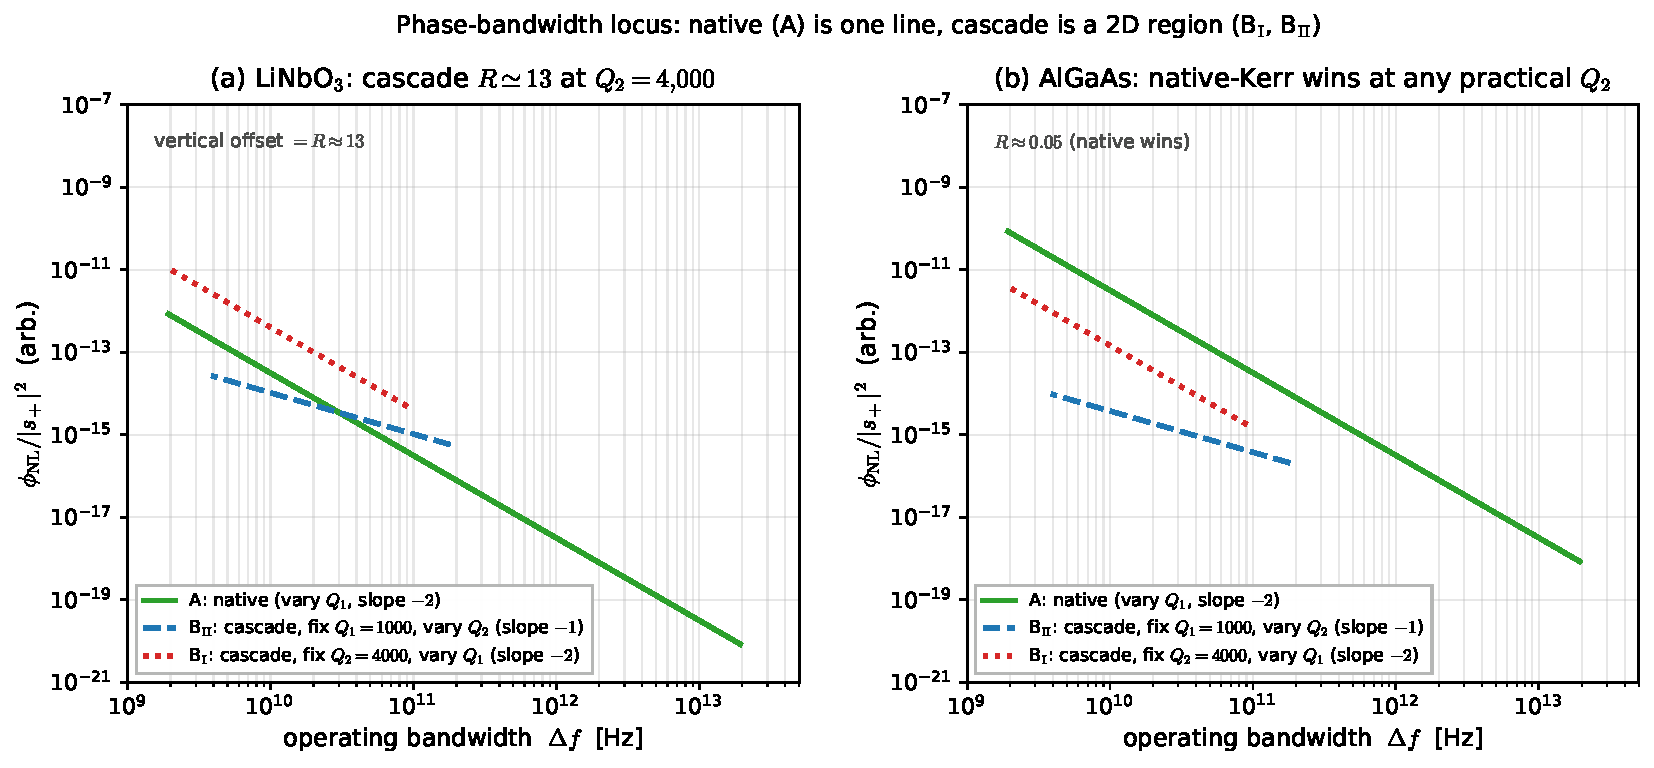
\includegraphics[width=\textwidth]{phase_shift_per_pump.pdf}
  \caption{Per-photon nonlinear phase shift versus operating bandwidth
  on log--log. Native (A, green solid, slope $-2$) is a single line.
  Cascade is a 2-D region bounded by B$_{\rm I}$ (red dotted,
  slope $-2$, parallel to A but vertically offset by $R$) and B$_{\rm II}$
  (blue dashed, slope $-1$, the sum-rule line). (a) LiNbO\textsubscript{3}:
  $R \approx 13$, cascade wins across the plotted range.
  (b) AlGaAs: $R \approx 0.05$, native wins.}
  \label{fig:phasebw}
\end{figure}

\paragraph{What is plotted.}
Per-photon phase scaling, three slope families (Section~11 of the note):
\begin{align}
  \text{A (native)}:\quad &
        \phi_{\rm NL}/|s_+|^{2} \propto Q_1^{2}\, \chithree_{\rm native},
        \quad \Delta f \propto 1/Q_1,
        \quad \text{slope}\,-2,\\
  \text{B}_{\rm II}\,(\text{fix }Q_1,\,\text{sweep }Q_2):\quad &
        \phi_{\rm NL}/|s_+|^{2} \propto Q_1^{2}\, Q_2\, \eta_\geom |\chitwo|^{2}/n_2^{2},
        \quad \Delta f \propto 1/Q_2,
        \quad \text{slope}\,-1,\\
  \text{B}_{\rm I}\,(\text{fix }Q_2,\,\text{sweep }Q_1):\quad &
        \phi_{\rm NL}/|s_+|^{2} \propto Q_1^{2} \cdot R(Q_2),
        \quad \Delta f \propto 1/Q_1,
        \quad \text{slope}\,-2.
\end{align}
B$_{\rm I}$ is parallel to A but vertically offset by the structural
ratio $R$ of \eqref{eq:Rdef}; B$_{\rm II}$ is the sum-rule locus.

\paragraph{Parameters.}
Both panels: $\eta_\geom = 0.3$, $\omega_1 = 1.22\!\times\!10^{15}$ rad/s,
$\Dom = 2\gamma_2$. Family A sweeps $Q_1 \in [10, 10^{5}]$; B$_{\rm II}$
fixes $Q_1 = 1\,000$, sweeps $Q_2 \in [100, 10^{5}]$; B$_{\rm I}$ fixes
$Q_2 = 4\,000$, sweeps $Q_1 \in [10, 10^{5}]$. Lines are truncated where
$\min(\gamma_1, \gamma_2)$ flips which decay rate is the bandwidth
bottleneck (the artificial cliffs in the unfiltered version).

\paragraph{Result.}
LiNbO\textsubscript{3}: B$_{\rm I}$ sits $R \approx 13\times$ above A
across the plotted range; B$_{\rm II}$ runs through them with slope
$-1$, intersecting A at very narrow bandwidth ($\sim$1\,GHz) that is
off the right edge of the experimentally relevant range. AlGaAs:
B$_{\rm I}$ sits $R \approx 0.05\times$ \emph{below} A; the cascade does
not compete at any practical bandwidth.

\paragraph{Interpretation.}
The cascade locus is a 2-D region, not a 1-D curve. Within it,
B$_{\rm II}$ is the slope-$-1$ \emph{sum rule} (Q$_2$-area conserved)
and B$_{\rm I}$ is a slope-$-2$ ladder of constant-$Q_2$ horizons.
Where the cascade region sits relative to the native line A is set
entirely by $R$: at $R \gg 1$ the cascade region floats above native,
at $R \ll 1$ it sinks below.

% --------------------------------------------------------------
\subsection{2-D design landscape}\label{sec:designmap}

\begin{figure}[H]
  \centering
  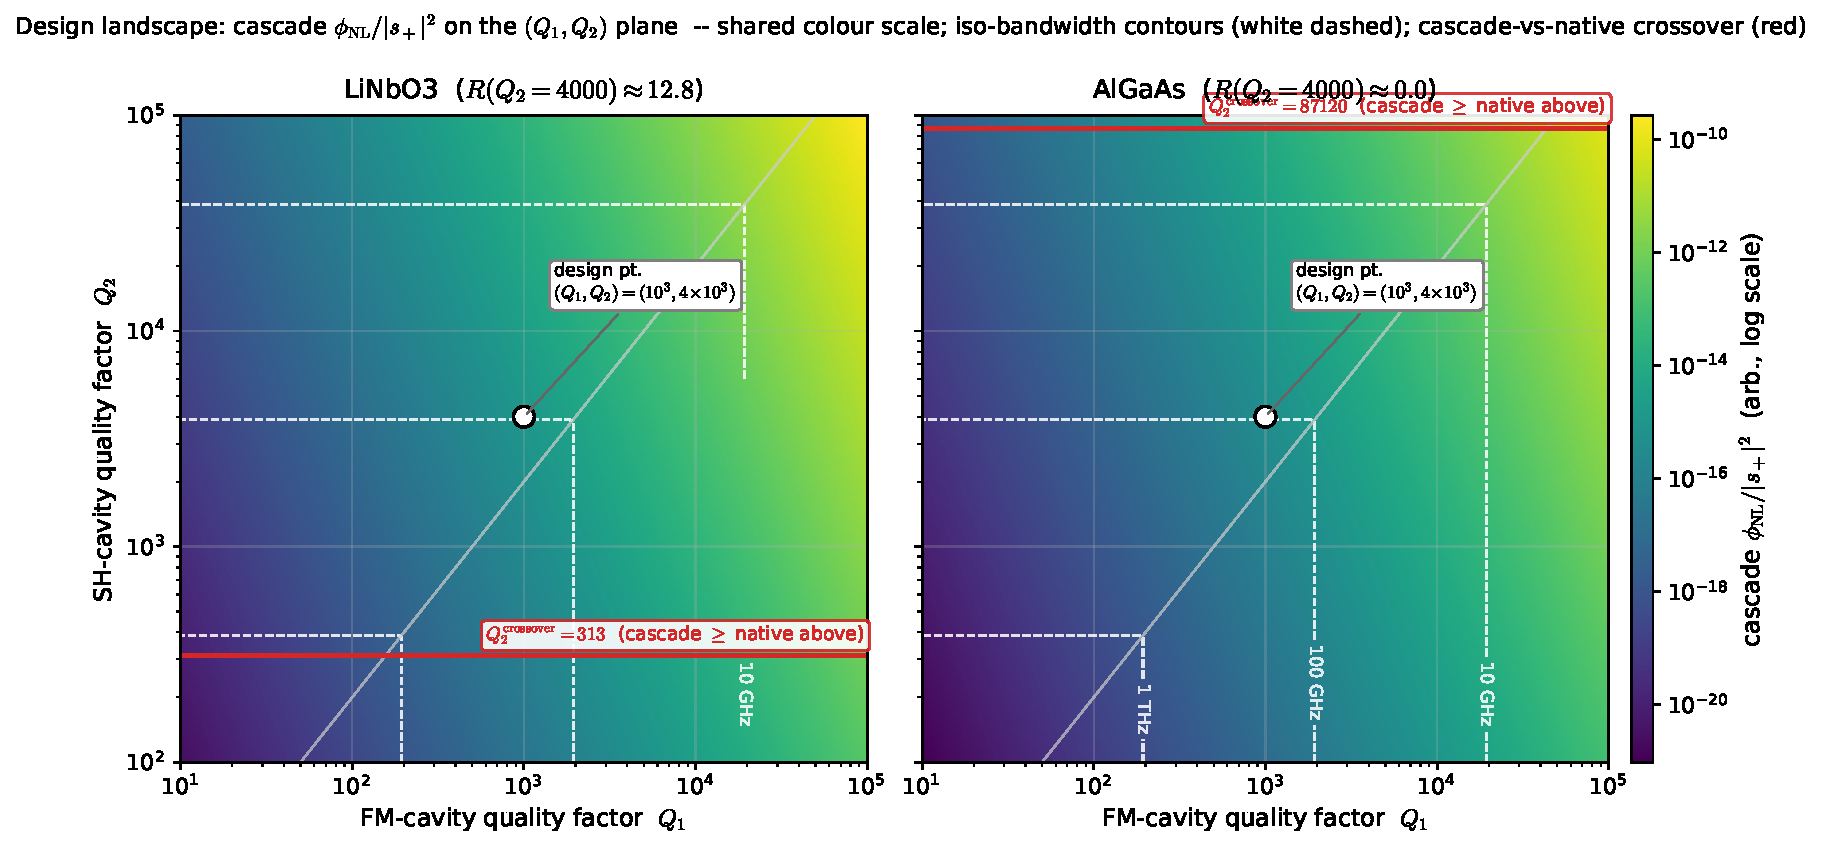
\includegraphics[width=\textwidth]{phase_shift_per_pump_2d.pdf}
  \caption{Cascade $\phi_{\rm NL}/|s_+|^{2}$ on the $(Q_1, Q_2)$ plane,
  shared colour scale across panels. White dashed contours: operating
  bandwidth $\Delta f = \min(\gamma_1, \gamma_2)/(2\pi)$. Red horizontal:
  $Q_2 = Q_2^{\rm crossover}$ (cascade $\geq$ native above). Grey
  diagonal: $Q_1 = Q_2/2$ (FM-bottleneck $\leftrightarrow$ SH-bottleneck
  boundary). White marker: design point $(Q_1, Q_2) = (10^{3}, 4\!\times\!10^{3})$.}
  \label{fig:designmap}
\end{figure}

\paragraph{What is plotted.}
For each host, the cascade per-photon phase
\begin{equation}
  \phi_{\rm NL}/|s_+|^{2} \;\propto\; Q_1^{2}\, Q_2\, \frac{|\chitwo|^{2}\,\eta_\geom}{n^{6}}
\end{equation}
as a colour heatmap on $(\log Q_1, \log Q_2)$. Three overlays:
(i) iso-bandwidth contours $\min(\gamma_1, \gamma_2) = $ const, which
form $\sf L$-shapes meeting at the diagonal $Q_1 = Q_2/2$;
(ii) the red line $Q_2 = Q_2^{\rm crossover}$ (above which cascade beats
native at every $Q_1$, by \eqref{eq:Rdef}); (iii) the LiNbO\textsubscript{3}
design point.

\paragraph{Parameters.}
$Q_1, Q_2 \in [10, 10^{5}] \times [10^{2}, 10^{5}]$ log-uniform on a
$220\times220$ grid; $\eta_\geom = 0.3$; LiNbO\textsubscript{3} and
AlGaAs material parameters from Table~\ref{tab:hosts}; shared colour
limits set to the min/max across both panels.

\paragraph{Result.}
LiNbO\textsubscript{3} (left): the red crossover line sits at $Q_2 = 156$
near the bottom edge; nearly the entire plotted $(Q_1, Q_2)$ rectangle
is in the cascade-wins region. The design point at $(10^{3}, 4\!\times\!10^{3})$
sits comfortably above the crossover. AlGaAs (right): the crossover line
sits at $Q_2 \approx 12\,600$, cutting the plot horizontally; the design
point at $(10^{3}, 4\!\times\!10^{3})$ falls \emph{below} -- native is
the right architecture there.

\paragraph{Interpretation.}
The 2-D map answers practical design questions in one figure: at a
chosen bandwidth target (an L-contour) and a chosen $Q$-budget (a
point), it reads off (a) the phase shift achievable with cascade,
(b) whether cascade or native is the better choice (above or below the
red line). The L-shaped bandwidth contours visualise the
sum-rule structure: along the vertical leg of each L, increasing $Q_2$
at fixed $Q_1$ buys phase at slope $-1$ in BW; along the horizontal
leg, increasing $Q_1$ at fixed $Q_2$ buys phase at slope $-2$ in BW.
Note the colour scale is host-dependent but \emph{shared} between
panels: LiNbO\textsubscript{3} is uniformly brighter than AlGaAs across
the plane because the $n^{-6}$ penalty in $\phi/{\rm pump}$ outweighs
the $|\chitwo|^{2}$ gain for high-index hosts.

% --------------------------------------------------------------
\subsection{Loss budget: the cascade-specific TPA penalty}\label{sec:lossbudget}

\begin{figure}[H]
  \centering
  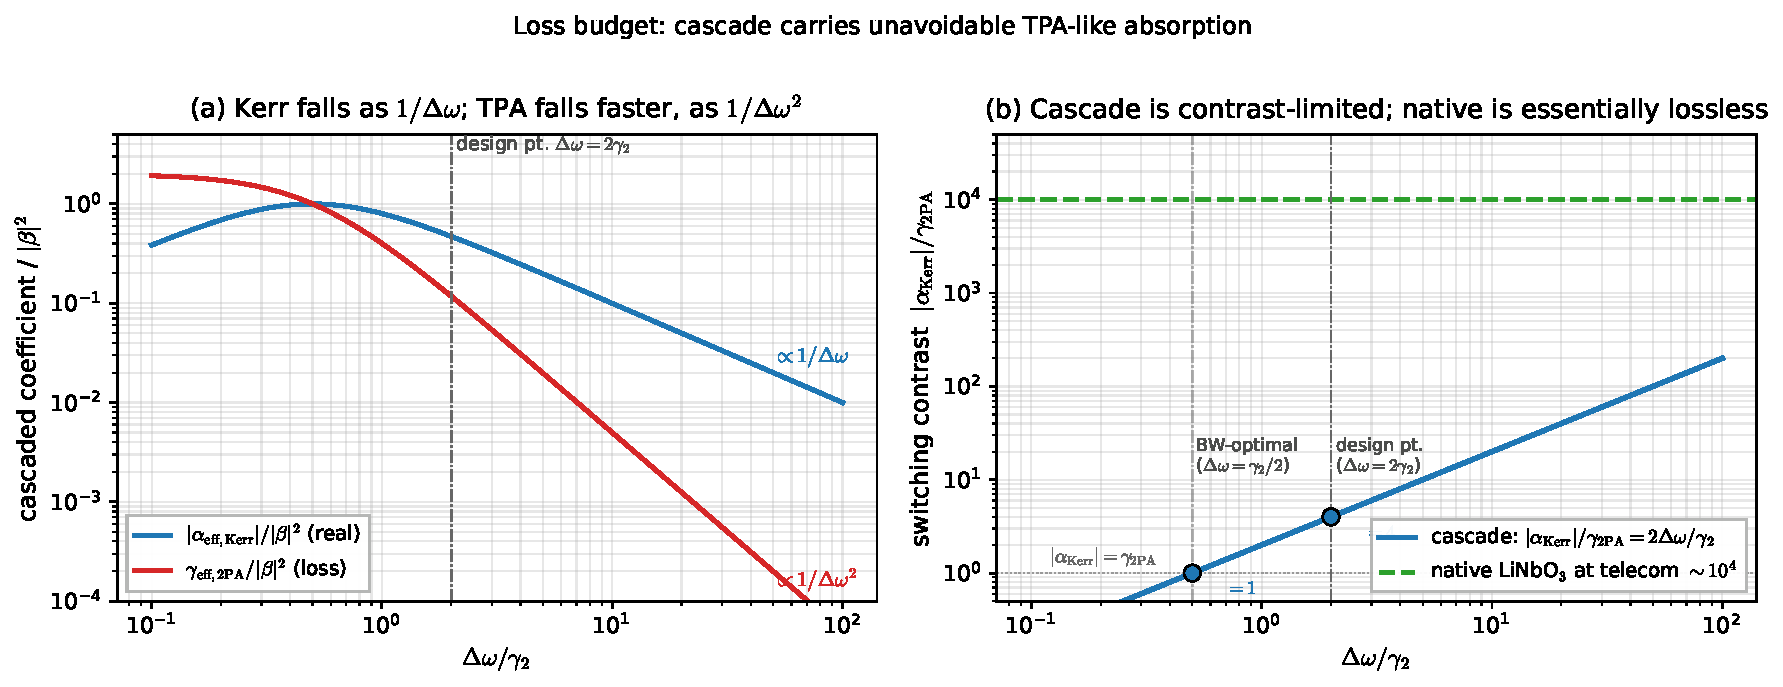
\includegraphics[width=\textwidth]{loss_budget.pdf}
  \caption{(a) Real (Kerr) and imaginary (TPA) parts of the cascaded
  coefficient vs.\ $\Dom/\gamma_2$. Kerr falls as $1/\Dom$
  (far-detuned); TPA falls faster, as $1/\Dom^{2}$, so contrast
  (Kerr/TPA) grows linearly with $\Dom$. (b) Cascade switching
  contrast $= 2\Dom/\gamma_2$ vs.\ $\Dom/\gamma_2$, compared with the
  native LiNbO\textsubscript{3} contrast at telecom ($\sim 10^{4}$,
  set by residual material absorption).}
  \label{fig:lossbudget}
\end{figure}

\paragraph{What is plotted.}
The cascaded coefficient on $|a_1|^{2} a_1$ in the FM equation is
complex; its real and imaginary parts (Kerr-like and TPA-like
respectively) are:
\begin{equation}
  \alpha_3^{\effc}
   = -\frac{|\beta|^{2}\, \Dom}{\Dom^{2} + (\gamma_2/2)^{2}},
  \qquad
  \gamma_{2{\rm PA}}^{\rm eff}
   = \frac{|\beta|^{2}\, (\gamma_2/2)}{\Dom^{2} + (\gamma_2/2)^{2}}.
\end{equation}
The contrast for switching is
\begin{equation}
  \frac{|\alpha_3^{\effc}|}{\gamma_{2{\rm PA}}^{\rm eff}}
   = \frac{2\Dom}{\gamma_2}.
  \label{eq:contrast}
\end{equation}

\paragraph{Parameters.}
$\Dom/\gamma_2 \in [0.1, 100]$ log-uniform; $\beta = \gamma_2 = 1$
(dimensionless TCMT). Native LiNbO\textsubscript{3} contrast estimate
$\sim 10^{4}$ taken from typical material data
($\chithree_{\rm native}/{\rm Im}\,\chithree_{\rm native}$ at 1550\,nm).

\paragraph{Result.}
At the bandwidth-optimal point $\Dom = \gamma_2/2$, contrast is exactly
unity (each rad of Kerr phase carries one rad of TPA absorption). At
the note's design point $\Dom = 2\gamma_2$, contrast is 4 (terrible,
relatively speaking). At far-detuned $\Dom = 10\gamma_2$, contrast is
20. Native LiNbO\textsubscript{3} sits $\sim 3$ orders of magnitude
higher.

\paragraph{Interpretation.}
The cascade carries an unavoidable absorption penalty that scales
linearly with the detuning. To raise the switching contrast, one must
push to far-detuned operation -- but \eqref{eq:Rdef} also shrinks as
$1/\Dom$, so contrast is bought at the cost of enhancement. The
sum-rule structure repeats here in disguise: cascaded TPA times
cascaded Kerr is invariant. For applications where extinction ratio
matters (all-optical switching, low-noise sensing), this contrast
ceiling is the cascade's most serious structural limitation, far more
than the saturation discussed in
\S\ref{sec:saturation}--\S\ref{sec:parametric_onset}.

% =====================================================================
\section{Summary of phenomena}
\label{sec:summary}

\begin{table}[H]
\centering
\renewcommand{\arraystretch}{1.20}
\setlength{\tabcolsep}{3pt}
\footnotesize
\begin{tabular}{>{\raggedright\arraybackslash}p{0.14\textwidth}
                >{\raggedright\arraybackslash}p{0.12\textwidth}
                >{\raggedright\arraybackslash}p{0.35\textwidth}
                >{\raggedright\arraybackslash}p{0.32\textwidth}}
\toprule
Phenomenon & Figure & Key formula & Practical implication \\
\midrule
Adiabatic Kerr & Fig.~\ref{fig:validation} &
$\alpha_3^{\effc} = -\DSH/[\DSH^{2}{+}(\gamma_2/2)^{2}]$ &
``$-1/\Dom$'' wrong near resonance \\
Sign tunability & Fig.~\ref{fig:sign_flip} &
$\alpha_3^{\effc}(-\Dom) = -\alpha_3^{\effc}(\Dom)$ &
Single device $\to$ focusing or defocusing \\
Sum rule & Fig.~\ref{fig:sumrule} &
peak $\times$ FWHM $= 2\sqrt{3}\,|\beta|^{2}$ &
$Q_2$ buys peak, not area \\
Bistability & Fig.~\ref{fig:bistability} &
cusp at $\delta_p > \sqrt{3}\, \gamma_1/2$ &
Cleanest CW signature \\
Saturation & Fig.~\ref{fig:saturation} &
$|\beta a_1| \to |\Dom|$ &
Max useful amplitude $\propto 1/Q_2$ (energy $\propto 1/Q_2^{2}$) \\
OPO onset & Fig.~\ref{fig:parametric_onset} &
trivial FP unstable at sat $\gtrsim 1$ &
Hard ceiling for the Kerr description \\
Pulse BW & Fig.~\ref{fig:pulse_bandwidth} &
adiabatic for $\sigma_t \gamma_2 \gtrsim 1$ &
Not for ultrafast \\
Manley--Rowe & Fig.~\ref{fig:manley_rowe} &
factor-of-2 in DFG essential &
Smoke test for any TCMT code \\
Bulk vs.~meta & Fig.~\ref{fig:bulk} &
shared sum-rule hyperbola &
0.5--1 dex in $\chithree$ traded for 2--3 dex in BW \\
Overlap & Fig.~\ref{fig:overlap} &
$\eta_\geom \in [10^{-3},\, 0.5]$ &
Geometry first \\
Index scaling & Fig.~\ref{fig:n2} &
$1/n_2^{2}$ not $1/n^{3}$ &
$\sim 2\times$ correction at telecom \\
Transmission & Fig.~\ref{fig:transmission} &
double-dip at high power &
Most diagnostic scan \\
\midrule
Arch.\ response & Fig.~\ref{fig:archresponse} &
$\phi_{\rm cas}/\phi_{\rm nat} = R \approx 12$ (numerical) &
Validates Section~11 of the note \\
Host survey & Fig.~\ref{fig:hostsurvey} &
$Q_2^{\rm cross}\propto n^{2}\chithree_{\rm nat}/|\chitwo|^{2}$ &
LiNbO\textsubscript{3} wins; AlGaAs loses \\
Phase-bandwidth & Fig.~\ref{fig:phasebw} &
Three slopes: A($-2$), B$_{\rm I}$($-2$), B$_{\rm II}$($-1$) &
Cascade is a 2-D region, native a 1-D line \\
Design map (2-D) & Fig.~\ref{fig:designmap} &
$(Q_1, Q_2)$ heatmap + iso-BW + crossover &
Visual design tool \\
Loss budget & Fig.~\ref{fig:lossbudget} &
Kerr/TPA contrast $= 2\Dom/\gamma_2$ &
Cascade contrast ceiling vs.\ native $\sim 10^{4}$ \\
\bottomrule
\end{tabular}
\caption{Phenomenon catalogue (the lower block lists the cascaded-vs-native
comparison figures of \S\ref{sec:comparison}).}
\label{tab:summary}
\end{table}

% =====================================================================
\section{Recommendations for metasurface design}
\label{sec:recommendations}

\subsection{Hierarchy of important parameters}

In order of decreasing leverage on $|\chithree_{\rm casc}|$:

\begin{enumerate}
\item $\eta_\geom$ -- three orders of magnitude separating poor and
  engineered overlap. Get this first; no amount of $Q_2$ rescues a
  vanishing tensor integral.
\item $|\chitwo|$ of the host material -- enters squared.
  Switching between LiNbO\textsubscript{3}, GaAs, AlGaAs is at most a
  factor of two; switching from a non-second-order material to
  LiNbO\textsubscript{3} is infinite.
\item $Q_2/n_2^{2}$ -- $1/n_2^{2}$ is fixed by material; $Q_2$ is
  engineered. A factor of two in $Q_2$ buys a factor of two in peak
  enhancement and a factor of $1/2$ in bandwidth.
\item $\Dom/\gamma_2$ -- operating point. The bandwidth-optimal point
  is $\Dom \sim \gamma_2/2$; far-detuned operation buys more
  pump-power headroom (saturation pushed up) at the cost of lower peak
  enhancement.
\item $\gamma_1/\gamma_2$ and $\grad/\gamma_1$ -- port coupling. Sets
  input efficiency; affects bistability threshold but not the cascaded
  coefficient itself.
\end{enumerate}

\subsection{Recommended design sequence}

\begin{enumerate}
\item Pick a non-centrosymmetric host with the largest $|\chitwo|$
  compatible with low loss in the FM and SH bands.
  LiNbO\textsubscript{3} at telecom is the standard; AlGaAs at near-IR
  has higher $|\chitwo|$ but higher absorption near the band edge.
\item Engineer the qBIC pair to maximise $\eta_\geom$. Use full-wave
  eigenmode simulation (COMSOL/MEEP) to compute the tensor overlap
  integral for candidate unit cells. Target $\eta_\geom \gtrsim 0.1$.
  Use periodic poling or geometry asymmetry to lift mode-parity
  constraints. Verify that $\eta_\geom$ stays high under realistic
  fabrication tolerances (lithography errors, sidewall angle).
\item Set $Q_2$ from the application's bandwidth requirement.
  $Q_2 \in [10^{3},\, 10^{5}]$ corresponds to
  $\Delta f \in [400\text{ GHz},\, 4\text{ GHz}]$. Higher $Q_2$ gives
  more enhancement, less bandwidth, and lower saturation power.
\item Set $\Dom$ near the bandwidth-optimal point
  $\Dom \sim \gamma_2$ for maximum enhancement, or further off-resonance
  ($\Dom \gtrsim 5\gamma_2$) for higher saturation power and easy
  sign-tunability through $\Dom = 0$.
\item Set $Q_1$ for input efficiency. $\grad/\gamma_1 \sim 0.5$
  (critically coupled) gives the deepest dip; under-coupled FM is
  fine if you have a strong source. Avoid over-coupled FM
  ($\grad > \gamma_1/2$, which is impossible since
  $\grad \le \gamma_1$ by definition; the relevant trap is
  $\grad/\gamma_1 \to 1$, where intrinsic $Q_1$ drops and dip width
  grows).
\item Verify that the pump power requirement does not exceed material
  damage thresholds. Saturation pump intensity scales as $1/\sqrt{Q_2}$
  at fixed $\Dom/\gamma_2$, so high-$Q$ designs saturate at low
  intensity. With $Q_2 = 10^{4}$ in LiNbO\textsubscript{3}, several
  MW/cm$^{2}$ in the resonator suffices for saturation, well within
  damage limits.
\end{enumerate}

\subsection{Trade-offs and optimisations}

\begin{table}[H]
\centering
\renewcommand{\arraystretch}{1.25}
\setlength{\tabcolsep}{4pt}
\footnotesize
\begin{tabular}{>{\raggedright\arraybackslash}p{0.27\textwidth}
                >{\raggedright\arraybackslash}p{0.31\textwidth}
                >{\raggedright\arraybackslash}p{0.33\textwidth}}
\toprule
You want\dots & Trade-off & How to mitigate \\
\midrule
Higher $|\chithree_{\rm casc}|$ &
narrower BW (sum rule); lower saturation; more thermal load per photon &
higher-$Q$ SH; active cooling; low-loss host
(LiNbO\textsubscript{3}) \\
Wider BW &
lower peak; more pump for the same nonlinear phase &
lower $Q_2$ or moderate $\eta_\geom$ at low $Q$ \\
Faster temporal response &
loses all cascaded enhancement at $\sigma_t \gamma_2 \lesssim 1$ &
switch to bulk phase-mismatched PPLN regime \\
Sign tunability without device swap &
fine $\Dom$ control required &
strain or thermo-optic tuning of the SH mode \\
Avoid parametric oscillation &
operate well below $|\beta a_1| \approx |\Dom|$ &
larger $\Dom$, lower input -- at lower phase shift \\
Avoid thermo-optic / free-carrier confusion &
loss leads to thermal heating &
LiNbO\textsubscript{3} (low absorption) over GaAs/Si near the band
edge \\
Suppress cascaded TPA &
TPA peaks at $\DSH = 0$; finite at any $\Dom$ &
operate at $|\Dom| \gtrsim 2\gamma_2$, where the imaginary part is
suppressed by $1/\DSH^{2}$ \\
\bottomrule
\end{tabular}
\caption{Practical trade-offs in metasurface design.}
\label{tab:tradeoffs}
\end{table}

\subsection{\texorpdfstring{Operating-point trade-off: aggressive vs.\ conservative $\Dom$}{Operating-point trade-off: aggressive vs. conservative Delta-omega}}\label{sec:tradeoff_R}

The note's worked example sits at $\Dom = 2\gamma_2$, giving
$R \simeq 12$ for LiNbO\textsubscript{3} at $Q_2 = 4{,}000$. The TCMT
figures of this report (Figs.~\ref{fig:archresponse},
\ref{fig:bistability}) use the same operating point and recover the
predicted $(1+R)$, $1/(1+R)$, and $(1+R)^{2}$ ratios to within a few
percent. Two alternative operating points are worth keeping in mind:

\begin{center}
\renewcommand{\arraystretch}{1.25}
\setlength{\tabcolsep}{4pt}
\footnotesize
\begin{tabular}{>{\raggedright\arraybackslash}p{0.15\textwidth}
                >{\raggedright\arraybackslash}p{0.09\textwidth}
                >{\raggedright\arraybackslash}p{0.26\textwidth}
                >{\raggedright\arraybackslash}p{0.37\textwidth}}
\toprule
$\Dom/\gamma_2$ & $R$ & Cascade strength & When to choose it \\
\midrule
$2$ (conservative) & $\sim 12$ &
moderate ($\alpha_3^{\rm casc} \approx 0.47$ in dim TCMT) &
\textbf{Default for narrowband CW devices.} Adiabatic SH elimination
is clean; TPA penalty suppressed by $(\gamma_2/2\Dom)^2 = 1/16$ vs.\
the Kerr; saturation cap $|a_1|^2 \approx 4$ leaves several decades
of linear pump range. \\
$1$ (edge of adiabatic) & $\sim 25$ &
strong ($\alpha_3^{\rm casc} \approx 0.80$) &
Pulls another factor of 2 in $R$, recovers the historical
``$R \sim 25$ for LiNbO\textsubscript{3}'' quote. The cost: the
adiabatic approximation $|\Dom| \gg \gamma_2/2$ becomes marginal;
TPA / Kerr ratio $\sim 0.5$; saturation cap halves. Use if you can
tolerate TPA loss and a narrower bistable / linear window. \\
$0.5$ (peak of $\alpha_3^{\rm casc}$) & $\sim 50$ &
maximum (peak Lorentzian, $\alpha_3^{\rm casc} = |\beta|^2/\gamma_2$) &
The mathematical maximum of the cascade-Kerr coefficient -- and the
peak of the cascaded-TPA loss simultaneously, with the two equal in
magnitude. Pure-SA regime; \emph{not} a Kerr operating point.
Useful for the saturable-absorber application (Fig.~\ref{fig:bistability}
companion: cascade SA), not for bistability / FWM / phase modulation. \\
\bottomrule
\end{tabular}
\end{center}

The Tier 1 ratios scale strictly as the relevant power of $(1+R)$
regardless of which operating point one picks, but the
\emph{absolute} magnitudes and the practically achievable linear pump
range differ.  Reproducing the figures in this report at $\Dom = \gamma_2$
amounts to halving $\widetilde\alpha_3$ from $0.04$ to $0.02$ in the
relevant scripts and adjusting the predicted $1+R$ accordingly.

The cleanest experimental statement is the cascade-vs-native ratio
itself, which is dimensionless and independent of the operating
point's absolute scale -- this is what Figs.~\ref{fig:archresponse}--%
\ref{fig:bistability} are designed to display.

\paragraph{Prefactor uncertainty (and what the numbers do not say).}
The $R$ values quoted throughout this report inherit an $O(1)$
multiplicative uncertainty from the convention dependence of the
modal coupling $\beta=(\eps_0\omega_1/4)\,M$ (see note \S5 discussion
preceding eq.~(beta)): the alternative $\eps_0\omega_1/2$ normalisation
would shift $|\beta|^{2}$ -- and therefore $R$ -- by a factor of $4$.
Together with the $\eta_\geom\!\sim\!0.3$ assumption, the absolute
$R$ values for LiNbO\textsubscript{3} ($R\!\sim\!12$ at the conservative
operating point) should be read as \emph{order-of-magnitude}
predictions.  Settling the prefactor requires a full-wave evaluation
of the modes and the overlap integral for a specific meta-atom design.
What is robust is the \emph{ratio} of cascade-to-native (which carries
the same prefactor in both) and the $Q$-scaling exponents.

\subsection{Plausible-looking ideas that do not work}

\begin{itemize}
\item \emph{Push $Q_2$ to $10^{6}$ for $1\,000\times$ enhancement.}
  Two reasons this fails: (i) the saturation pump amplitude drops
  as $1/Q_2$ (and the stored-energy cap as $1/Q_2^{\,2}$), so the
  peak enhancement is unreachable at any practical input; (ii) at
  $Q_2 = 10^{6}$, the SH linewidth is $\sim 40$ MHz, and sub-nm
  fabrication errors detune resonators randomly across the array,
  smearing the metasurface response back to a low-effective-$Q$
  regime.
\item \emph{Add the bulk Kerr for free.} The bulk $|\chithree|$ in
  LiNbO\textsubscript{3} is $\sim 2 \!\times\! 10^{-21}$
  m$^{2}$/V$^{2}$, $\sim 12\times$ below the cascaded value at the
  conservative operating point. The bulk contribution is a few-percent
  correction at the design point; it only matters near the
  zero-crossing of the total Kerr (Fig.~\ref{fig:sign_flip}, red
  curve).
\item \emph{Add gain to push past the OPO threshold.} Above threshold
  the system \emph{is} an OPO, not a Kerr medium. Useful for
  parametric source design, not for the cascaded-$\chithree$ use cases
  this note targets.
\end{itemize}

% =====================================================================
\section{Open issues}
\label{sec:open}

\begin{itemize}
\item \emph{Tensor structure of $\chitwo_{ijk}$.} The simulations use
  a scalar $\beta$. A real metasurface has a tensorial $\chitwo_{ijk}$
  contracted with vectorial mode profiles. Different polarisation
  channels give different $\beta$; signs and magnitudes can differ
  across channels. Full-wave simulation is needed for a quantitative
  number.
\item \emph{Disorder / inhomogeneous broadening.} Lithographic disorder
  broadens $\gamma_2$ inhomogeneously: the array linewidth is
  $\gamma_2^{\rm array}\!\simeq\!\sqrt{\gamma_2^{2}+\sigma_{\omega_2}^{2}}$,
  and the cascaded enhancement is set by $Q_2^{\rm array}$, not the
  element $Q_2$. For $Q_2^{\rm element}\!\sim\!10^{4}$ at telecom,
  preserving the cascade requires $\sigma_{\omega_2}/\omega_2\!\lesssim\!10^{-4}$
  (sub-nm geometric control). See note \S13 item 7 for mitigations
  (post-fab trimming, electro-optic feedback). The TCMT model assumes
  a single resonator; for an array, the homogeneous response we
  simulate must be convolved with this distribution.
\item \emph{Thermo-optic and free-carrier nonlinearities.} Note \S13
  item 4 flags these as easy to confuse with Kerr at the intensities
  required ($\sim$MW/cm$^{2}$); not modelled here.
\item \emph{Vector mode profiles in $\eta_\geom$.}
  Fig.~\ref{fig:overlap} treats $\eta_\geom$ as a free parameter; the
  actual value comes from a full-wave eigenmode integration that we
  have not done.
\end{itemize}

% =====================================================================
\section{Code reference}
\label{sec:code}

\begin{table}[H]
\centering
\small
\begin{tabular}{>{\raggedright\arraybackslash}p{0.27\textwidth}
                >{\raggedright\arraybackslash}p{0.65\textwidth}}
\toprule
File & Purpose \\
\midrule
\texttt{tcmt.py} & Core TCMT integrator (DOP853, complex packing) \\
\texttt{analytic.py} & Closed-form expressions: $\alpha_3^{\effc}$,
$\gamma_{2{\rm PA}}^{\rm eff}$, Kerr-only cubic, $a_2$ adiabatic \\
\texttt{params.py} & \texttt{TCMTParams} dataclass plus
LiNbO\textsubscript{3} reference numbers \\
\texttt{style.py} & Shared matplotlib rcParams and palette \\
\texttt{fig\_*.py} & One per phenomenon (17 in total, including the
   five comparison figures of \S\ref{sec:comparison}) \\
\texttt{linear\_stability.py} & 4$\times$4 Jacobian eigenvalues of the
   trivial fixed point (used by \texttt{fig\_parametric\_onset.py}) \\
\texttt{run\_all.py} & Driver \\
\bottomrule
\end{tabular}
\caption{Files in \texttt{cascaded\_chi3/}.}
\label{tab:code}
\end{table}

To regenerate every figure:
\begin{verbatim}
conda run -n ml_base python run_all.py
\end{verbatim}

% =====================================================================
\section{Cross-reference to the note}
\label{sec:cross}

\begin{itemize}[nosep]
\item Polarisation-tensor derivation: \S4 (note)
\item TCMT equations: \S5 (note)
\item $\beta$ formula: eq.~(beta), \S5 (note)
\item Adiabatic elimination and $\alpha_3^{\effc}$: \S6(i)
\item Cascaded TPA: \S6(ii)
\item Sum rule: \S7
\item Tensor and phase-matching constraints: \S8
\item BIC/qBIC platforms: \S9
\item LiNbO\textsubscript{3} worked example: \S10
\item Cascaded-vs-native architectural comparison: \S11 (note) --
      directly mirrored by \S\ref{sec:comparison} of this report
\item Application landscape (saturable absorber, AM modulator,
      optical limiter, $\Dom$-sensor): \S12 (note)
\item Validity regions, including disorder/inhomogeneous broadening: \S13
\item Boxed final result: eqs.~(chi3casc), (chi3casc\_explicit)
\end{itemize}

\end{document}
